\documentclass[journal]{IEEEtran}

% *** FLOAT PACKAGES ***
%
%\usepackage{fixltx2e}
% fixltx2e, the successor to the earlier fix2col.sty, was written by
% Frank Mittelbach and David Carlisle. This package corrects a few problems
% in the LaTeX2e kernel, the most notable of which is that in current
% LaTeX2e releases, the ordering of single and double column floats is not
% guaranteed to be preserved. Thus, an unpatched LaTeX2e can allow a
% single column figure to be placed prior to an earlier double column
% figure.
% Be aware that LaTeX2e kernels dated 2015 and later have fixltx2e.sty's
% corrections already built into the system in which case a warning will
% be issued if an attempt is made to load fixltx2e.sty as it is no longer
% needed.
% The latest version and documentation can be found at:
% http://www.ctan.org/pkg/fixltx2e


%\usepackage{stfloats}
% stfloats.sty was written by Sigitas Tolusis. This package gives LaTeX2e
% the ability to do double column floats at the bottom of the page as well
% as the top. (e.g., "\begin{figure*}[!b]" is not normally possible in
% LaTeX2e). It also provides a command:
%\fnbelowfloat
% to enable the placement of footnotes below bottom floats (the standard
% LaTeX2e kernel puts them above bottom floats). This is an invasive package
% which rewrites many portions of the LaTeX2e float routines. It may not work
% with other packages that modify the LaTeX2e float routines. The latest
% version and documentation can be obtained at:
% http://www.ctan.org/pkg/stfloats
% Do not use the stfloats baselinefloat ability as the IEEE does not allow
% \baselineskip to stretch. Authors submitting work to the IEEE should note
% that the IEEE rarely uses double column equations and that authors should try
% to avoid such use. Do not be tempted to use the cuted.sty or midfloat.sty
% packages (also by Sigitas Tolusis) as the IEEE does not format its papers in
% such ways.
% Do not attempt to use stfloats with fixltx2e as they are incompatible.
% Instead, use Morten Hogholm'a dblfloatfix which combines the features
% of both fixltx2e and stfloats:
%
% \usepackage{dblfloatfix}
% The latest version can be found at:
% http://www.ctan.org/pkg/dblfloatfix

% Citation package
\usepackage{cite}

% graphic package
\ifCLASSINFOpdf
  \usepackage[pdftex]{graphicx}
  \DeclareGraphicsExtensions{.pdf,.jpeg,.png}
\else
  % \usepackage[dvips]{graphicx}
  % \DeclareGraphicsExtensions{.eps}
\fi

% math package
\usepackage{amsmath,amsfonts,amssymb,amscd,amsthm,xspace}
\usepackage{array}

% subfigure package
\ifCLASSOPTIONcompsoc
  \usepackage[caption=false,font=footnotesize,labelfont=sf,textfont=sf]{subfig}
\else
  \usepackage[caption=false,font=footnotesize]{subfig}
\fi

% tikz for graphs
%\usepackage{tikz}
%\usetikzlibrary{arrows,shapes,snakes,automata,backgrounds,petri, calc}

% other necesssary packages
\usepackage{multirow}
\usepackage{times}
% \usepackage{subcaption}
% \usepackage[pdf]{graphviz}

\usepackage{breqn}
\usepackage{hyperref}

% correct bad hyphenation here
\hyphenation{spe-ci-fi-cal-ly re-gu-la-ted ge-ne-ra-li-sa-ti-on fun-ding dif-fe-rent pa-ra-me-ter a-ve-ra-ging ha-ving bia-ses va-lu-es in-fe-ren-ce theo-rem pro-ba-bi-li-ty ap-pro-xi-ma-ti-on ma-xi-mi-sing u-sing e-le-ments de-fi-ni-ti-on}

\DeclareMathOperator*{\argmax}{arg\,max}

\begin{document}

% some symbols for easy calls
\newcommand{\tp}{\textrm{\textit{tp}}}
\newcommand{\fp}{\textrm{\textit{fp}}}
\newcommand{\tpr}{\textrm{\textit{tpr}}}
\newcommand{\fnr}{\textrm{\textit{fnr}}}
\newcommand{\fpr}{\textrm{\textit{fpr}}}
\newcommand{\tnr}{\textrm{\textit{tnr}}}
\newtheorem{definition2}[subsection]{Definition}

% \title{Partially Observable Count Estimation by an Autonomous Mobile Robot}
\title{Count on Me: Partially Observable Poisson Processes applied to Mobile Robot Exploration}
% \title{Spectral-POPP for Robot Exploration in Partially Observable Environments}

\author{Ferdian~Jovan, Milan Tomy Mariya, Jeremy Wyatt, Nick Hawes 
% \IEEEcompsocitemizethanks{\IEEEcompsocthanksitem F. Jovan is with the Department
% of Engineering Science, University of Oxford, Oxford, OX1~3PJ.\protect\\
% E-mail: ferdian.jovan@gmail.com 
% \IEEEcompsocthanksitem Jeremy Wyatt is with the Department of Computer Science, University of Birmingham, Birmingham, B15~2TT.
% \IEEEcompsocthanksitem Nick Hawes is with Oxford Robotics Institute, Oxford, OX2~6NN. 
% }% <-this % stops an unwanted space
% \thanks{Manuscript received April 19, 2005; revised August 26, 2015.}
}

% The paper headers
\markboth{IEEE TRANSACTIONS ON ROBOTICS, VOL. XX, NO. X, MONTH YEAR}%
{Shell \MakeLowercase{\textit{et al.}}: Bare Demo of IEEEtran.cls for IEEE Journals}

% make the title area
\maketitle

\begin{abstract}
    The Poisson assumption is a popular choice when data arises in the form of counts. In many applications such as in mobile robotics, such counts are prone to a systematic error due to unreliable sensor algorithms and the data set that result can not be trusted. Only limited works have been done on the Poisson model when a full observability of the data is in question. We present practical Bayesian estimators in this paper for a partially observable Poisson process (POPP). Variations of these processes are presented, in which (i) sensors are uncorrelated, (ii) sensors are correlated, (iii) the unreliability of the observation model, when built from data, is accounted for. The actual posterior distributions are estimated via two tractable approximations, which we combined in a switching filter. The filter enables efficient and accurate estimation of the posterior. A detailed empirical analysis is performed on both simulated and real-world data, and an application of the resulting posterior to drive exploration of a mobile robot with unreliable sensors is presented. 
\end{abstract}

\begin{IEEEkeywords}
Poisson processes, partial observability, misclassified counts, robot exploration
\end{IEEEkeywords}


\IEEEpeerreviewmaketitle

\section{Introduction}
\label{sec:introduction}

In recent years, autonomous mobile robots have started to come to assist humans with simple daily tasks in our homes and offices \cite{hawes2016strands}. As the robot is expected to work in dynamic environments, any behaviour model for the robot to adapt with humans is typically learnt over time from observations \cite{coppola2016learning}. Where these observations are made using sensor data, both humans and all the currently robotic sensory systems have some level of unreliability. This means collected data-sets that make up the observations typically contain systematic errors that lead to bias in the statistical estimate produced by the sensors. In this paper, we address the unreliability problem of sensors counting events by formulating a \textit{partially observable Poisson process} (POPP). As we may require it do so for when multiple sensors are involved in which one sensor may (or may not) correlate to one another, we extend the POPP model with several variations. A standard fully observable Poisson process (FOPP) is introduced to distinct the POPP and its derivatives from it.

Several practical contributions are made. First, a set of inference methods for a Poisson process which take into account the unreliability of either single or multiple sensory systems used to count events is addressed. Two tractable approximations to the posterior of such Poisson processes, which are combined into a switching filter, are presented to cope with the absence of a conjugate density. One (the \textit{Gamma filter}) is fast, but prone to drift from the true posterior in certain circumstances. The second (the \textit{histogram filter}) is slower but avoids drifts. Variations of these processes are introduced. First is the correlated POPP (C-POPP) to deal with sensors that are correlated to one another. The second variation is the POPP-Beta which deals with the unreliability of the observation model. We also combine the C-POPP and the POPP-Beta in the POPP-Dirichlet model that is able to deal with correlated sensors and the unreliability of the observation model. We demonstrate the properties of the POPP, its variations, and its filters by numerical simulations and real-world datasets.

Finally, we show the benefit of the POPP model, and its variation on a robot exploration task performed by a mobile robot. The resulting posterior of the POPP and its derivative is used to drive exporation by a mobile robot for a series of two week deployment. Robot exploration rises from the fact that any mobile robot needs to observe human activities/behaviour in order to learn and adapt in its human-populated environment. As the robot has a limit to its operational life, one would therefore like it to optimise the time it takes to build its models. We contrast this with an exploration method based on the FOPP model. We show that the exploration method involving corrections to systematic errors doubles the number of human encounters the robot experiences. 

% We show variations of the exploration methods based on optimistic predictions from the resulting posteriors of the first contribution. 
% BELUM BERES INI
% The second contribution is the variation of exploration methods for a mobile robot based on optimistic predictions from the resulting posteriors of the first contribution. As any mobile robot in human-populated environment needs to learn human behaviour/activity, it must first explore where activities are likely to happened and observe them. One would like the robot to observe a sufficient amount of human activity, so as to learn the specific kinds of activity models. However, as a mobile robot can only be in one place at one time, its observations are spatially restricted. Moreover, the robot has a limit to its operational life. We would therefore like it to optimise the time it takes to build its models. This introduces an exploration-exploitation trade-off problem \cite{wyatt1998exploration, 1413255, AUDIBERT20091876}, i.e. should the robot visit a familiar place, where it will probably observe two activities, or go to a new place, where it might observe many more but might see nothing? 

% is expected to work around and/or with humans, modelling human activities becomes a necessity. In any scenario where a robot learns about human activities, it must first explore where activities are likely to happened and observe them. 
% 
% One would like the robot to observe a sufficient amount of human activity, so as to learn the specific kinds of activity models. However, as a mobile robot can only be in one place at one time, its observations are spatially restricted. Moreover, the robot has a limit to its operational life. We would therefore like it to optimise the time it takes to build its models. This introduces an exploration-exploitation trade-off problem \cite{wyatt1998exploration, 1413255, AUDIBERT20091876}, i.e. should the robot visit a familiar place, where it will probably observe two activities, or go to a new place, where it might observe many more but might see nothing?
% 
% Another important restriction in mobile robotics is that robot sensors are unreliable. Any solution must take into account the unreliability of sensors. We may also require that it do so for when multiple sensors are involved. This means that collected data which are used for learning typically contain systematic errors that lead to bias in the statistical estimates produced by the event detection processes.

% To allow the robot to observe a sufficient amount of human activity, so as to learn the specific kinds of activity models, putting an exploration to places with high number of activities becomes a mandatory action. There are several reasons behind this. First, a mobile robot can only be in one place at one time, so its observations are spatially restricted.   
% 
% The problem of this thesis can be loosely formulated as how to predict where many people are most likely to be and to go and observe them. Specifically, it requires the robot to go to where the aggregate level of human activity is highest. In addition, this thesis chooses to tackle the problem for the case where the robot runs for an extended period of time such days, or even weeks as it builds its models.
% A key challenge is for the robot to be able to recognise and react adequately to dynamic changes that happen in human-centered environments, especially when the changes are the result of human behaviour. The learning process for an autonomous mobile robot to adapt to its environment takes a big portion of its lifetime and it needs to deal with the huge volume of experiences accessible to it as it runs for longer periods of time. One advantage of all these is that these experiences contain potentially useful information that can help the robot to eventually adapt to its environment.

% Taken together, the challenges and benefits faced by an autonomous mobile robot motivate this thesis to create long-term understanding of temporal dynamics of human activities, along with the ability to exploit this understanding for a better adaptation of an autonomous mobile robot. The robot is expected to demonstrate its ability to predict future activities based on its statistical model. It is also expected to be able to detect anomalies as sequences of very low likelihood data.



%!TEX root = ../bare_jrnl.tex

\section{Fully Observable Poisson Process}
\label{sec:preliminaries}

A \emph{fully observable} Poisson process (FOPP) models the distribution of $N(t)$, the number of events appearing in time interval $[0, t)$, parameterised by an \textit{arrival rate}, $\lambda$:
\begin{equation}
    \label{eq:pmf_poisson}
	Poi(N(t) = c \mid \lambda) = \frac{e ^{-\lambda} \lambda ^{c}}{c!}
\end{equation}
We use $N(t) = c_i$ to refer to a count recorded during the $i$-th observation of the process.
Given a Gamma density
\begin{equation}
    \label{eq:pdf_gamma}
    \begin{tabular}{rcl}
        $Gam(\lambda \mid \alpha, \beta)$ & = & $\displaystyle\frac{\beta ^{\alpha}}{\Gamma (\alpha)} \lambda ^{\alpha - 1} e^{-\beta \lambda}$ \\ [1ex]
    \end{tabular}
\end{equation}
as a prior distribution over the parameter $\lambda$, where $\alpha, \beta$ are the shape and the rate parameters, the posterior over $\lambda$ for a FOPP can be  calculated via Bayesian inference with
\begin{equation}
    \label{eq:posterior_fopp}
    \begin{array}{lll}
        P(\lambda \mid c_1, \ldots, c_n) & \varpropto Poi(c_1, \ldots, c_n \mid \lambda) ~ Gam(\lambda \mid \alpha, \beta) \\
         & = Gam \Bigg(\lambda \Bigm| \displaystyle\sum_{i=1}^{n} \alpha + c_i, \beta + n \Bigg)
    \end{array}
\end{equation}
This adds the sample counts $\sum_{i=1}^{n} c_i$ to the hyper-parameter $\alpha$ of the gamma prior, and adds the number of observations $n$ to the hyper-parameter $\beta$ of the gamma prior.

The FOPP model requires a single reliable sensor. With an unreliable sensor, FOPP inferences will be incorrect.
\section{Related Work}
\label{sec:related}

There are some existing works which address statistical models where the observation data are not fully observable. In some literature, this effect is regarded as misclassified counts. Misclassification happens when there are false positive counts or false negative counts (or possibly both). False positive counts, which can also be called the overcount, are when the count includes events other than those of interest. Whereas false negative counts, which can also be called the undercount, are when some of the events of interest are missed or omitted. Early work on this involving count data dealt with the undercount (or under-reporting) problem as this is quite a common problem. Whittemore and Gong estimated cervical cancer rates by taking into account false negative data \cite{whittemore1991}. Winkelmann and Zimmermann introduced a combination of a Poisson regression model with a logit model for under-reporting, yielding the Poisson-Logistic (Pogit) model \cite{winkelmann1993poisson}. They applied this to model the number of days employees were absent from a workplace. Dvorzak and Wagner borrowed the Pogit model and incorporated a small set of validation data, which is assumed available, to provide information about the true counts \cite{dvorzak2016}. A Bayesian analysis of the Poisson-Logistic model was performed and Bayesian variable selection was incorporated to identify regressors with a non-zero effect and also to restrict parameters of the Poisson-Logistic model.

Fewer worked on the Poisson model in the case when the count data may either be undercounting or overcounting \cite{sposto1992, bratcher2002, bratcher2004, stamey2005}. Sposto et al. estimated both cancer and non-cancer death rates, assuming false negatives are possible on both sides of these counts \cite{sposto1992}. The approach used by them followed the frequentist framework. Bratcher and Stamey, in \cite{bratcher2002}, used a Bayesian method to estimate Poisson rates in the presence of both undercounts and overcounts borrowing the double sampling technique introduced in \cite{Tenenbein1970}. They then extended their work to a fully Bayesian method for interval prediction of the unobservable actual count in future samples, given a current double sample \cite{bratcher2004}. Stamey and Young \cite{stamey2005} managed to obtained closed-form expressions for maximum likelihood estimators of the false negative rate, the false positive rate, and the Poisson rate for the model proposed in \cite{bratcher2002}. The estimators are straightforward to calculate and to interpret in terms of evaluating the effectiveness of using unreliable counts.

Our work is similar to the work in \cite{bratcher2002} to accurately estimate the parameter of a single Poisson process. They utilised the double sampling technique to obtain the true count together with false positive count and false negative count. The Poisson rate is estimated via an MCMC approximation due to no-closed form and expensive calculation of the posterior distribution of $\lambda$. Our work differs from theirs in that they are interested in estimation of a single Poisson process where the estimation is based on two counters with one always being a perfect counter. Here, we consider multiple unreliable counters, which may have correlations to one another, applied to estimating the parameter of a single Poisson process. To tackle the non-trivial density of the posterior, three precise and tractable Bayesian estimators are proposed. 

Our work is actually an extension to the work in \cite{jovan18a} in accurately estimating the parameter of a single Poisson process to improve its prediction accuracy. We present three further extensions of the original model presented in \cite{jovan18a} and their applications to exploit the temporal dynamics in the aggregate level of human activities for better robot exploration.

% involved binomial and multinomial models \cite{Bross1954,Chen1979,Hochberg1977,Tenenbein1970,Viana1993}. The first technique which was recorded to handle misclassification was double sampling. It was first introduced by Tenenbein to correct for misclassification of binomial data and obtain a maximum likelihood estimate \cite{Tenenbein1970}. The double sampling approach utilizes two search techniques to retrieve relevant information: an expensive classification technique to obtain the true count along with the false positive count and false negative count from typically a small sample set, and a less-expensive classification technique only for error-prone counts on a larger sample set. The results of both counts are then combined to obtain estimators for the Poisson rate $\lambda$, and also for the misclassification parameters. The work of Tenenbein was then extended by Chen \cite{Chen1979} and Hochberg \cite{Hochberg1977} to correct misclassified counts in categorical and multinomial models to obtain maximum likelihood estimates. The double sampling technique was also extended to incorporate prior distributions in the binomial model and the posterior was obtained via Bayesian estimation \cite{Viana1993}. Bekele extended the work of \cite{Viana1993} by introducing a weighted prior scheme and allowing for several sources of information, including expert opinions \cite{bekele1998binomial}.

% Different than the case of binomial and multinomial models, only a few studies are found working on the effect of partial observability of the data on the Poisson distribution. Many deal 

\section{The POP Process}
\label{sec:popp}

The partially observable Poisson process (POPP) is a counting process $N(t)$ with arrival rate $\lambda$ where the number of events that occurred up to time $t$ are obtained by unreliable (possibly multiple) counters. The definition brings a distinction between \emph{true count} (or simply \emph{count}), which refers to the number of events that actually happened, and the \emph{sensed count}, which refers to the count obtained by a counter (or sensor). Given that $c_i$ number of events happened (as the true count) over the interval $[0, t)$ during the $i$-th observation, and $m$ counters observed the events unreliably, thus the sensed count $s_{ji}$ is the count given by sensor $j$ in the $i$-th observation within the interval $[0, t)$ with $0 \leq j \leq m$. 

\begin{figure}[t!]
	\centering
	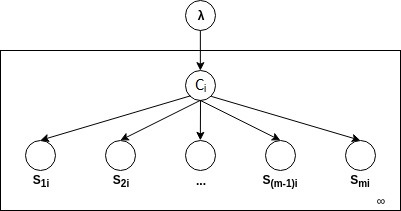
\includegraphics[width=0.5\textwidth]{./figures/gm_popp.jpg}
    \caption{Graphical representation of the partially observable Poisson process.}
	\label{fig:gm_popp}
\end{figure}

The graphical model, which is easily derived from the definition of the POPP, shows that the true count $c_i$ has become a latent variable which can only be inferred from the sensed count $\overrightarrow{s_i} = (s_{1i}, \ldots, s_{mi})$ where each $s_{ji}$ is a sensed count coming from sensor $j$. The posterior of $\lambda$ is then inferred from the posterior of $c_i$ after multiple samples $i = 1 \ldots n$.

A statistical inference to estimate the rate parameter $\lambda$ of the POPP model is done with a marginalisation over all possible true count value $c_i$ in a joint distribution between the posterior $P(\lambda ; c_i)$ and the posterior over $c_i$ given $\overrightarrow{s_i}$. The posterior of $\lambda$, given $n$ samples $\overrightarrow{s}=(\overrightarrow{s_1} \dots \overrightarrow{s_n})$, each consisting of $m$ sensors, is:
\begin{equation}
	\label{eq:marginal_occurrences}
	\begin{tabular}{r@{=}l}
		$P(\lambda ; \overrightarrow{s})$ &  $\displaystyle\sum_{c_1=0}^{\infty} \ldots \displaystyle\sum_{c_n=0}^{\infty} P(\lambda ; \overrightarrow{c}) ~ P(\overrightarrow{c} ; \overrightarrow{s})$ \\
	\end{tabular}
\end{equation}
\noindent where
\begin{equation*}
	\begin{tabular}{r@{ = }l}
		$P(\lambda ; \overrightarrow{c})$ & $Gam\Bigg(\lambda ; \displaystyle\sum_{i=1}^{n} c_i + \alpha, n + \beta \Bigg)$
	\end{tabular}
\end{equation*}
\noindent with $\overrightarrow{c} = (c_1, \ldots, c_n)$ for $1 \leq i \leq n$.

$P(\overrightarrow{c} ; \overrightarrow{s})$ is factored based on the assumption that each sensor is \textit{uncorrelated} to one another given the true count $c_i$. Consequently, the probability that the vector of true counts is $\overrightarrow{c}$, given $n$ samples of the vector of $m$ sensed counts $\overrightarrow{s_1}, \ldots, \overrightarrow{s_n}$, is

\begin{equation}
    \label{eq:occurrences_likelihood}
    \begin{tabular}{r@{ $\varpropto$ }l}
        $P(\overrightarrow{c} ; \overrightarrow{s_1}, \ldots, \overrightarrow{s_n})$ & $P(\overrightarrow{s_1}, \ldots, \overrightarrow{s_n} ; \overrightarrow{c}) ~ P(\overrightarrow{c})$ \\ [1ex]
        & $\displaystyle\prod_{i=1}^{n} P(\overrightarrow{s_i} ; c_i) ~ P(c_i)$ \\ [2ex]
        & $\displaystyle\prod_{i=1}^{n} \displaystyle\prod_{j=1}^{m} P(s_{ji} ; c_i) ~ P(c_i ; \overrightarrow{c_{-1}})$
    \end{tabular}
\end{equation}

\noindent where $\overrightarrow{c_{-1}} = c_{i-1}, \ldots, c_1$.

$P(c_i ; \overrightarrow{c_{-1}})$ and $P(s_{ji} ; c_i)$ are defined to complete Eqn. \ref{eq:occurrences_likelihood}. $P(c_i ; \overrightarrow{c_{-1}})$ is calculated in the form of a negative binomial distribution

\begin{equation}
	\label{eq:unconditional_xi}
	\begin{tabular}{r@{=}l}
		$P(c_i ; \overrightarrow{c_{-1}})$ & $\displaystyle\int_{\lambda=0}^{\infty} P(c_i ; \lambda) ~ P(\lambda ; \overrightarrow{c_{-1}}) ~d\lambda$ \\ [2ex]
		& $\displaystyle\int_{\lambda=0}^{\infty} Poi(c_i ; \lambda) ~ Gam(\lambda ; \alpha, \beta) ~d\lambda$ \\ [2ex]
		& $NB\Bigg(c_i ; \alpha, \displaystyle\frac{\beta}{\beta + 1}\Bigg)$.
	\end{tabular}
\end{equation}

The Poisson limit theorem states that the Poisson distribution may be used as an approximation to the binomial distribution \cite{papoulis2002probability}. Using this theorem as the foundation, an arbitrarily close approximation to the probability $P(s_{ji} ; c_i)$ is defined by assuming there exists a small enough finite subinterval of length $\delta$ for which the probability of more than one event occurring is less than some small value $ \epsilon$. With this assumption, interval $[0, t)$ is splitted into $l$ smaller subintervals $I_1, \ldots, I_l$ of equal size, with the condition that $l > \lambda$ (the condition is crucial since we focus on very small portions of the interval). Consequently, the whole interval $[0, t) = I_1, \ldots, I_l$ becomes a series of Bernoulli trials, where the $k^{th}$ trial corresponds to whether (1) an event $e_k$ happens with probability $\lambda / l$ and (2) a sensor $j$ captures the event $e_k$ as the detection $d_k$ at the subinterval $I_k$.

$P(s_{ji} ; c_i)$ is defined as the aggregate of the true positives $tp_{ji}$ in $c_i$ subintervals, and the false positives $fp_{ji}$ in $l-c_i$ subintervals. The probability of a \textit{true positive detection} (TP) for sensor $j$ in a subinterval is $tpr_j = P_j(d = 1 ; e=1)$, and the probability of a \textit{false positive detection} (FP) is $fpr_j = P_j(d = 1 ; e=0)$. Thus $P(s_{ji} ; c_i)$ is defined as a sum of two binomial distributions $B(r ; n,\pi)$, where the aggregate is constrained to be $s_{ji}$: 

\begin{equation}
	\label{eq:joint_binomial_distribution}
    P(s_{ji} ; c_i) \! = \! \! \! \displaystyle\sum_{\textrm{tp}_{ji} = 0}^{c_{i}} \! \! B\Big(\textrm{tp}_{ji} ; c_i, \textrm{tpr}_j\Big) B\Big(\textrm{fp}_{ji} ; \Delta c_i, \textrm{fpr}_j \Big)
\end{equation}
\noindent where $s_{ji} = \textrm{tp}_{ji} + \textrm{fp}_{ji}$, $\textrm{tpr}_j = P_j(d=1 ; e=1)$, $\textrm{fpr}_j = P_j(d=1 ; e=0)$, and $\Delta c_i = (l - c_i)$.

Eqn.~\ref{eq:marginal_occurrences} shows the difficulty of belief state estimation in the POPP model since there is no conjugate density accomodating an analytical solution for the posterior over $\lambda$. Each sensed count sample $\overrightarrow{s_i}$ used to update the posterior of $\lambda$ adds a factor of countably infinite number of elements. The resulting posterior is a sum of countably infinite sums. One can place an upper bound $l$ on the maximum value of each $c_i$, but it still makes the number of elements in the posterior grow by a factor $l$ with every sensed count $\overrightarrow{s_i}$.  

With this difficulty noted, Jovan et al., proposed three efficient estimators, each of which offers an approximation to the true posterior $P(\lambda ; \overrightarrow{s})$. A more detailed presentation of these estimators is given in \cite{jovan18a}.

% \input{src/filter.tex}
\subsection{The POPP-Beta}
\label{subsec:popb}

In the POPP model, an observation model is represented as a confusion matrix which specifies the true positive rate (sensitivity)--along with its false negative rate--and the true negative rate (specificity)--along with its false positive rate. To construct a confusion matrix, one needs to have both sensed counts and the ground truth, i.e. the true counts. Typically, the sensed counts and their true counts need expert labelling to pre-process them before they can be used to train an observation model. As expected, the POPP model requires the observation model to be accurate to prevent posteriors over $\lambda$ to infer incorrect inferences. However, attaining an accurate observation model requires a lot of training data and this puts a lot of burden on the experts who need to label the data.   

Here, we extended the POPP model in a different direction than the one shown in the C-POPP model. The observation model is transformed into a Bayesian estimation problem where each element in the confusion matrix, (true positive rate ($\tpr$) and false positive rate ($\fpr$)), follows a beta distribution. Beta distributions are chosen for $\tpr$ and $\fpr$ because Beta distributions act as a conjugate to Binomial distributions and provide a family of prior probability distributions for the parameter of a binomial distribution. The beta-binomial conjugacy leads to an analytically tractable compound distribution called the beta-binomial distribution, where the $p$ parameter in the binomial distribution $B(d ; x, p)$ is randomly drawn from a beta distribution $Be(p ; \zeta, \eta)$.

\begin{equation}
	\label{eq:beta_binomial}
	\begin{tabular}{r@{ = }l}
		$P(d ; c, \zeta, \eta)$ & $\displaystyle\int_{0}^{1} P(d ; c, p) ~ P(p ; \zeta, \eta) ~dp$ \\ [2ex]
		& $\displaystyle\int_{0}^{1} B(d ; c, p) ~ Be(p ; \zeta, \eta) ~dp$ \\ [2ex]
        & $\displaystyle\int_{0}^{1} \binom{c}{d} p^d (1-p)^{(c-d)} ~ \displaystyle\frac{p^{(\zeta - 1)} (1-p)^{(\eta-1)}}{\pi(\zeta, \eta)}$ \\ [2ex]
        & $\displaystyle\binom cd \displaystyle\frac{1}{\pi(\zeta, \eta)} \displaystyle\int_{0}^{1} p^{(d+\zeta-1)} (1-p)^{(c-d+\eta-1)} dp$ \\ [2ex]
        & $\displaystyle\binom cd \displaystyle\frac{\pi(d+\zeta, c-d+\eta)}{\pi(\zeta, \eta)}$ \\ [2ex]
        & $BB(d ; c, \zeta, \eta)$
	\end{tabular}
\end{equation}

As the confusion matrix is now in the form of two beta distributions $Be(\tpr ; \zeta_{\tpr}, \eta_{\tpr})$ and $Be(\fpr ; \zeta_{\fpr}, \eta_{\fpr})$, $\zeta_{\tpr}$ can be thought as the number of true positive detections $\#(d=1, e=1)$, $\eta_{\tpr}$ as the number of false negative detections $\#(d=0, e=1)$, $\zeta_{\fpr}$ as the number of false positive detection $\#(d=1, e=0)$, and $\eta_{\fpr}$ as the number of true negative detections $\#(d=0, e=0)$ that the sensor has made. Given a confusion matrix where the elements of it follow beta density, and beta-binomial distributions which provide an unconditional distribution of $d$, Eqn. \ref{eq:joint_binomial_distribution} is now replaced with:  

\begin{equation}
	\label{eq:joint_beta_binomial_distribution}
    P(s_{ji} ; c_i) \! = \! \! \! \displaystyle\sum_{\tp_{ji} = 0}^{x_{i}} \! \! ~ BB\Big(\tp_{ji} ; c_i, \Phi_j \Big) BB\Big(\fp_{ji} ; \Delta c_i, \Psi_j \Big)
\end{equation}
\noindent where $s_{ji}= \tp_{ji} + \fp_{ji},~\Phi_j = (\tpr_{j}, \fnr_{j}),~\Psi_j = (\fpr_j, \tnr_j),~\tpr_j = \#_j(d=1, e=1),~ \fnr_j = \#_j(d=0, e=1),~\fpr_j = \#_j(d=1, e=0),~\tnr_j = \#_j(d=0, e=0)$, and $\Delta c_i = (l - c_i)$.

% With a sensor model which follows beta densities and is fully integrated, as a distribution, in the sensed count likelihood $P(s_{ji} ; c_i)$ as shown in Equation \ref{eq:joint_beta_binomial_distribution}, we obtain a graphical model with the structure shown in Figure \ref{fig:gm_popp_beta}.

One should note that the difference between the POPP model and this variation, which we call the POPP-Beta model, lies only on Eqn. \ref{eq:joint_binomial_distribution} and \ref{eq:joint_beta_binomial_distribution}. However, given little training data for the observation model, the POPP-Beta model is expected to be more conservative in estimating the posterior $P(\lambda ; \overrightarrow{s})$ over $\lambda$ than the POPP model. 

% \begin{figure*}[t!]
% 	\centering
% 	\begin{tikzpicture}
% 	\tikzstyle{place}=[rectangle,draw=blue,thick,minimum size=5 mm]
% 	\tikzstyle{empty}=[rectangle,draw=white,thick,minimum size=5 mm]
% 	\tikzstyle{every label}=[black]
% 	\begin{scope}
% 	\node[place](31)[xshift=0mm]{$S_{1i}$};
% 	\node[place](32)[right of=31, xshift=20mm]{$S_{2i}$};
% 	\node[place](33)[right of=32, xshift=20mm]{$\ldots$};
% 	\node[place](34)[right of=33, xshift=20mm]{$S_{(m-1)i}$};
% 	\node[place](35)[right of=34, xshift=22mm]{$S_{mi}$};
% 	\node[place](21)[above of=33]{$X_i$} edge[post](31) edge[post](32) edge[post](33) edge[post](34) edge[post](35);
% 	\node[place](11)[above of=21]{$\lambda$} edge[post](21);
%     \node[place](12)[right of=11, xshift=20mm]{$\textrm{tpr}_{(m-1)}, \textrm{fpr}_{(m-1)}$} edge[post](34);
%     \node[place](13)[left of=11, xshift=-20mm]{$\textrm{tpr}_{2}, \textrm{fpr}_{2}$} edge[post](32);
%     \node[place](14)[right of=12, xshift=22mm]{$\textrm{tpr}_{m}, \textrm{fpr}_{m}$} edge[post](35);
%     \node[place](15)[left of=13, xshift=-20mm]{$\textrm{tpr}_{1}, \textrm{fpr}_{1}$} edge[post](31);
% 	\node[empty](01)[above of=11]{};
%     \node[place](02)[above of=12]{$(\zeta, \eta)_{\textrm{tpr}}, (\zeta, \eta)_{\textrm{fpr}}$} edge[post](12);
%     \node[place](03)[above of=13]{$(\zeta, \eta)_{\textrm{tpr}}, (\zeta, \eta)_{\textrm{fpr}}$} edge[post](13);
%     \node[place](04)[above of=14]{$(\zeta, \eta)_{\textrm{tpr}}, (\zeta, \eta)_{\textrm{fpr}}$} edge[post](14);
%     \node[place](05)[above of=15]{$(\zeta, \eta)_{\textrm{tpr}}, (\zeta, \eta)_{\textrm{fpr}}$} edge[post](15);
% 	\end{scope}
% 	\end{tikzpicture}
%     \caption{Graphical representation of the POPP-Beta.}
% 	\label{fig:gm_popp_beta}
% \end{figure*}

%!TEX root = ../bare_jrnl.tex

\subsection{The Correlated POPP}
\label{subsec:cpop}

Recall that Eqn.~\ref{eq:occurrences_likelihood} is defined under the assumption that each sensor count is conditionally independent from all the others given the true count. This assumption ignores the correlations between sensors. 
% 
To introduce correlations between sensors we must alter Eqn.~\ref{eq:independent_sensor_likelihood} and
Eqn.~\ref{eq:joint_binomial_distribution} from the POPP model.


Recall that the probability of a particular sensed count given the true count $P(\mathbf{s_i} ; c_i)$ was defined from the Poisson limit theorem as a sequence of Bernoulli trials over $l$ subintervals. With correlated sensors, the observation of an event $e_k$ in the $k^{th}$ trial no longer follows the Bernoulli distribution. Instead it follows the categorical distribution, where the $k^{th}$ trial corresponds to whether a particular combination of binary detections $d_{1,k}, \ldots, d_{m,k}$ happens in subinterval $I_k$. Therefore, to replace Eqn.~\ref{eq:joint_binomial_distribution}, we propose to define the probability of a series of detection outcomes given the true count $c_i$ at interval $i$ as the following.

We first define for some interval $i$, $l$ subintervals, and $m$ sensors, there is a binary matrix of detections $\mathbf{D^i}$ (We drop the ($i$) for all notations in this subsection as we will consider a single interval). $\mathbf{D} \in \mathcal{D}^{m , l}$ the set of binary matrices of dimension $m \times l$. Each column $k$ of $\mathbf{D}$, we denote $\mathbf{D}_{:k} = \mathbf{d} = \{0, 1\}^m$ with $k = 1, \ldots, l$. Therefore, $\mathbf{D}$ is a series of $m$ sensor detections for $l$ subintervals, and $\mathbf{D_{:k}}$ is a vector of detections from $m$ different sensors at particular subinterval $k$. It should be clear by now that we move our notation from using $s_{j, i}$ representing sensed counts for particular sensor $j$ independently at time interval $i$ to $\mathbf D^{i}$ representing a series of $m$ sensor detections together at time interval $i$.

We further define $e_k \in \{0, 1\}$ as the variable indicating whether or not an event is hypothesized to have occurred in sub-interval $k$. $e_k = 1$ means that an event occurred. We define $P^{+}$ as the categorical distribution of $\mathbf{d}$, conditioned on $e = 1$, i.e.
\begin{equation}
	\label{eq:joint_sensor_model_positive_event}
	P^+(\mathbf{d}) = P(\mathbf{d} ; e = 1) ~~~~~ \forall \mathbf{d} \in \{0, 1\}^m
\end{equation} 
\noindent and, by analogy,
\begin{equation}
	\label{eq:joint_sensor_model_negative_event}
	P^-(\mathbf{d}) = P(\mathbf{d} ; e = 0) ~~~~~ \forall \mathbf{d} \in \{0, 1\}^m
\end{equation}
\noindent Both $P^+$ and $P^-$ have $2^m$ elements. These two probabilities represent \textit{true positive detection} and \textit{true negative detection}  similar to $\tau$ and $\xi$ for the POPP model.

We can partition the subintervals $1, \ldots, l$ into two sets. $\mathbf{e}^+$ is the set of subintervals $k$ where $e_k = 1$, and $\mathbf{e}^-$ is the set of subintervals $k$ where $e_k = 0$. We can define a partition of the subintervals by a pair $(\mathbf{e}^+, \mathbf{e}^-)$. The set of possible partitions such that $\mathbf{e}^+$ has a fixed size $c$, i.e. $\mid \mathbf{e}^+ \mid = c$, is denoted $\Sigma_c$, so that $(\mathbf{e}^+, \mathbf{e}^-) \in \Sigma_c$.

We further define $\mathbf{D}_{\mathbf{e}^+}$ as an $m \times c$ detection matrix formed from all the columns $\mathbf{D}_{:k}$ where $k \in \mathbf{e}^+$, and $\mathbf{D}_{\mathbf{e}^-}$ as the corresponding $m \times (l - c)$ detection matrix formed from all the columns $\mathbf{D}_{:k}$ where $k \in \mathbf{e}^-$.

As there may be duplicate columns in either or both $\mathbf{D}_{\mathbf{e}^+}$ and $\mathbf{D}_{\mathbf{e}^-}$, we define a count vector for each.
\begin{equation*}
	\mathbf{g}^+ = \textrm{count}(D_{\mathbf{e}^+})
\end{equation*}
\noindent and
\begin{equation*}
	\mathbf{g}^- = \textrm{count}(D_{\mathbf{e}^-})
\end{equation*}
\noindent such that $\sum\limits_{q=1}^{2^m} g_q^+ + \sum\limits_{r=1}^{2^m} g_r^- = l$ where each of $\mathbf{g}^+, \mathbf{g}^-$ are of length $2^m$, having one element for every possible detection vector $\mathbf{d} \in \{0, 1\}^m$.

In order to define the joint probability of a particular count being yielded by a particular sequence of detection outcomes, we must consider all possible combinations of true positives and false positives that could be generated by that sequence by exploring all elements of $\Sigma_c$. We do this in the following definition of $P(\mathbf{D} ; c)$, and define the probability of a given sequence of detection groups yielding count $c$ using the multinomial distribution.

\begin{equation}
\label{eq:codependent_sensor_likelihood}
P(\mathbf{D} ; c) = \sum\limits_{(\mathbf{e}^+, \mathbf{e}^-) \in \Sigma_c} Multi(\mathbf{g}^+ ; c, P^+) ~ Multi(\mathbf{g}^- ; (l - c), P^-)
\end{equation}

Eqn.~\ref{eq:codependent_sensor_likelihood} can be understood by analogy to Eqn.~\ref{eq:joint_binomial_distribution}. In both equations all possible ways pairs of true and false positives counts which sum to $c$ are considered. In the conditionally independent case the binomial distribution is used to determine the probability of each count from the available trials given the true and false positive rates. In the correlated case the multinomial distribution is used to determine the probability of each count from a possible sequence of joint observations and their probability of yielding a count.

One should note that the benefit of C-POPP is that it exploits correlations among multiple sensors contributing to detection counts. If there is only one sensor counting events, then the POPP model is more computationally efficient.


%\subsection{The Correlated POPP}
%\label{subsec:cpop}
%
%Recall that Eqn.~\ref{eq:occurrences_likelihood} is defined under the assumption that each sensor count is conditionally independent from all the others given the true count. This assumption ignores the correlations between sensors. 
%% 
%To introduce correlations between sensors we must alter Eqn.~\ref{eq:independent_sensor_likelihood} and
%Eqn.~\ref{eq:joint_binomial_distribution} from the POPP model.
%
%
%To replace Eqn.~\ref{eq:joint_binomial_distribution}, recall that the probability of a particular sensed count was defined from the Poisson limit theorem as a sequence of Bernoulli trials over $l$ subintervals.
%% 
%With correlated sensors, the observation of an event $e_k$ in the 
%$k^{th}$ trial no longer follows the Bernoulli distribution. Instead it follows the categorical distribution, where the $k^{th}$ trial corresponds to whether a particular combination of binary detections $d_{1,k}, \ldots, d_{m,k}$ happens in subinterval $I_k$. Therefore, instead of having independent sensor models for the detection of event $e_k$ we propose the joint observation model:
%\begin{equation}
%\label{eq:joint_sensor_model}
%P_{jnt}(\mathbf{d_k} ; e_k)
%\end{equation}    
%\noindent where $ \mathbf{d_k} = (d_{1,k}, \ldots, d_{m,k})$, with $d_{j,k}$ being a detection by sensor $j$ in the $k^{th}$ subinterval, and $d_{j,k}, e_k \in {0, 1}$. 
%
%From this we define functions $\mathcal E^+, \mathcal E^- : \mathbf{d} \rightarrow [0,1]$ which provide the probability of a joint observation given that $e_k$ occurred or did not, respectively. 
%
%\begin{equation}
%\mathcal E^+ = P_{jnt}(\mathbf{d_k} ; e_k=1)
%\end{equation}
%\begin{equation}
%\mathcal E^- = P_{jnt}(\mathbf{d_k} ; e_k=0)
%\end{equation}
%
%
%% \textbf{NOTE: Probably not needed but this implies that the value of each function over all $\mathbf{d_k}$ sums to 1. \emph{$\mathcal E^+$ and $\mathcal E^-$, each sums up to 1. These $\mathcal E^+$ and $\mathcal E^-$ are basically the TPR and TNR in these joint observation/sensor models}}
%
%Recall that the set of detections for observation period $i$ was defined as:
%\begin{equation*}
%\mathbf{s_i} = (s_{1i}, \ldots, s_{mi})
%\end{equation*}
%with $s_{j,i} \in \mathbb N$, the sensed count of sensor $j$ from the $i$-th observation period. Since the joint observation model is defined under a combination of binary detections of sensors, each $s_{j,i}$ can be split into $l$ subintervals such that in each sub interval $I_k$ there is only one detection $d_{j,k}$. If the binary detections from all sensors at subinterval $I_k$ are grouped together, then for the observation period $i$, $\mathbf{s_i}$ can be alternatively defined as a list of $l$ \emph{detection groups} of binary detections:
%\begin{equation}
%\label{eq:s_i_definition}
%\mathbf{s'_i} = ((d_{1,1}, \ldots, d_{m,1}), \ldots, (d_{1,l}, \ldots, d_{m,l}))
%\end{equation}
%\noindent with $d_{j,k}$ being a detection by sensor $j$ at subinterval $I_k$ and $d_{j,k} \in \{0, 1\}$. 
%% Note that this is not a set since detection groups can be duplicated across subintervals.
%
%In order to define the joint probability of a particular count being yielded by a particular sequence of detection groups, we must consider all possible combinations of true positives and false positives that could be generated by that sequence. We do this in the following definition of $P(\mathbf{s_i} ; c_i)$, and define the probability of a given sequence of detection groups yielding count $c_i$ using the multinomial distribution.
%
%\begin{equation}
%\label{eq:codependent_sensor_likelihood}
%P(\mathbf{s_i} ; c_i) = \sum\limits_{\mathbf{s} \in \mathcal{P}(\mathbf{s'_i})} Multi(\mathbf{s} ; |\mathbf{s}|, \mathcal E^+) ~ Multi(\mathbf{s'_i}\setminus \mathbf{s} ; (c_i - |\mathbf{s}|), \mathcal E^-)
%\end{equation}
%
%\noindent where $\mathcal{P}(\mathbf{s'_i}) = 2^{\mathbf{s'_i}}$, i.e. the list all possible combinations of size $n$ from of elements of $s'_i$\footnote{We have used the powerset symbol, $\mathcal{P}$, since it provides an indication of the entity being created. However note that we are not working with sets since $\mathbf{s'_i}$ can contain multiple identical sequences of $d_{j,k}$.}. 
%
%% \textbf{NOTE: \emph{Is using powerset correct? How do we distinguish the total number of each $(d_{1,1}, \ldots, d_{m,1}$?}}
%
%Eqn.~\ref{eq:codependent_sensor_likelihood} can be understood by analogy to Eqn.~\ref{eq:joint_binomial_distribution}. In both equations all possible ways pairs of true and false positives counts which sum to $c_i$ are considered. In the conditionally independent case the binomial distribution is used to determine the probability of each count from the available trials given the true and false positive rates. In the correlated case the multinomial distribution is used to determine the probability of each count from a possible sequence of joint observations and their probability of yielding a count.
%
%One should note that the benefit of C-POPP is that it exploits correlations among multiple sensors contributing to detection counts. If there is only one sensor counting events, then the POPP model is more computationally efficient.

%!TEX root = ../bare_jrnl.tex

\subsection{The POPP-Dirichlet}
\label{subsec:popd}

The C-POPP model uses a joint observation model in estimating the parameter $\lambda$ of a Poisson process. A joint observation model is an extension of an observation model where the model provides a probability for a particular combination of binary detections coming from each sensor given the true event as show in Eqn. \ref{eq:joint_sensor_model}.

To construct a joint observation model, one needs to have both detections and the corresponding actual (non-)event as ground truth. Pre-processing involving expert interventions is typically required before the detections and their corresponding ground truth can be further used. Similar to the POPP model, the C-POPP model requires the joint observation model to be accurate to avoid the posterior over $\lambda$ drifting away from the true posterior. If attaining an accurate observation model for the POPP model is a problem, then this becomes more prominent in the case of a joint observation model. This is because the training data needed to construct a joint observation model grows by a factor of two for each sensor involved.       

Similar to the extension from the POPP model to the POPP-Beta model, we can extend the C-POPP joint observation model into a Bayesian estimation problem. In this case the joint observation models ($P_{jnt}(d_{1,k}, \ldots, d_{m,k} ; e_k = 1)$ and $P_{jnt}(d_{1,k}, \ldots, d_{m,k} ; e_k = 0)$) will follow Dirichlet distributions. The Dirichlet distribution is an appropriate distribution since $P_{jnt}$ sets the probabilities of multinomial distributions in Eqn. \ref{eq:codependent_sensor_likelihood} and Dirichlet distributions provide a family of prior probability distributions for the multinomial distribution. The Dirichlet-multinomial conjugacy leads to an analytically tractable compound distribution which is called the Dirichlet-multinomial distribution, where the $\mathbf{p} = (p_1, \ldots, p_r)$ parameter in the multinomial distribution $Multi(\mathbf{d} ; c, \mathbf{p})$ is randomly drawn from a Dirichlet distribution $Dir(\mathbf{p} ; \mathbf{\zeta})$. 

\begin{equation}
	\label{eq:beta_binomial_revisit}
	\begin{tabular}{r@{ = }l}
        $P(\mathbf{d} ; c, \mathbf{\zeta})$ & $\displaystyle\int P(\mathbf{d} ; c, \mathbf{p}) ~ P(\mathbf{p} ; \mathbf{\zeta}) ~d\mathbb S_r$ \\ [2ex]
        & $\displaystyle\int Multi(\mathbf{d} ; c, \mathbf{p}) ~ Dir(\mathbf{p} ; \mathbf{\zeta}) ~d\mathbb S_r$ \\ [2ex]
        & $DM((d_1, \ldots, d_r) ; c, (\zeta_1, \ldots, \zeta_r))$
	\end{tabular}
\end{equation}
\noindent with $\mathbf{d} = (d_1, \ldots, d_r)$, $\mathbf{\zeta} = (\zeta_1, \ldots, \zeta_r)$, and $d\mathbb S_r$ denotes integrating $\mathbf{p}$ with respect to the $(r - 1)$ simplex\footnote{The support of the Dirichlet distribution is the $(r - 1)$-dimensional simplex $\mathbb S_r$; that is, all $r$ dimensional vectors which form a valid probability distribution}.

Given $m$ sensors, a joint observation model is now represented as two Dirichlet distributions: $Dir(\mathcal{E^+} ; \mathbf{\zeta^+})$, and $Dir(\mathcal{E^-} ; \mathbf{\zeta^-})$ with $\mathbf{\zeta^+} = (\zeta^+_0, \ldots, \zeta^+_{(m^2)-1})$ and $\mathbf{\zeta^-} = (\zeta^-_0, \ldots, \zeta^-_{(m^2)-1})$. $\mathbf{\zeta^+}$ and $\mathbf{\zeta^-}$ set the overall shape of the Dirichlet priors, with each $\zeta_q$ term counting the number of times that particular combination of sensor detections were produced given a positive ($\mathbf{\zeta^+}$, $e=1$) or negative ($\mathbf{\zeta^-}$, $e=0$) detection.


Given a joint sensor model where its elements follow a Dirichlet density and several Dirichlet-multinomial distributions, which provide an unconditional distribution of $(d_1, \ldots, d_r)$, we replace Eqn. \ref{eq:codependent_sensor_likelihood} with:  

\begin{equation}
	\label{eq:joint_dirichlet_multinomial_distribution}
    \begin{tabular}{r@{=}l}
		$P(\mathbf{s_i} ; c_i)$ & $\displaystyle\sum_{\mathbf{s} \in \mathcal{P}(\mathbf{s'_i})} DM(\mathbf{s} ; |\mathbf{s}|, \mathbf{\zeta^+}) ~ DM(\mathbf{s'_i}\setminus\mathbf{s} ; (l - |\mathbf{s}|), \mathbf{\zeta^-})$
	\end{tabular}
\end{equation}
\noindent with $s'_i$ and $\mathcal{P}$ as defined in Section~\ref{subsec:cpop}.

% With a joint sensor model following the Dirichlet density, which is conjugated with multinomial distributions into a posterior predictive distribution shown in Eqn. \ref{eq:joint_dirichlet_multinomial_distribution}, a graphical model is shown in Figure \ref{fig:gm_popp_dirichlet}.

The difference between the C-POPP model and the POPP-Dirichlet lies only in Eqn. \ref{eq:codependent_sensor_likelihood} being replaced by \ref{eq:joint_dirichlet_multinomial_distribution}. However, given a certain Dirichlet prior, and limited training data for the sensor model, the POPP-Dirichlet is expected to be more conservative in estimating the posterior $P(\lambda \mid \mathbf{s})$ over $\lambda$ than the C-POPP model.

% \begin{figure}[t!]
% 	\centering
% 	\begin{tikzpicture}
% 	\tikzstyle{place}=[rectangle,draw=blue,thick,minimum size=5 mm]
% 	\tikzstyle{every label}=[black]
% 	\begin{scope}
%     \node[place](51)[xshift=30mm]{$(\zeta^+_0, \ldots, \zeta^+_{(m^2)-1})$};
%     \node[place](52)[right of=51, xshift=30mm]{$(\zeta^-_0, \ldots, \zeta^-_{(m^2)-1})$};
%     \node[place](41)[above of=51, yshift=3mm]{$(E^+_0, \ldots, E^+_{(m^2)-1})$} edge[pre](51);
%     \node[place](42)[above of=52, yshift=3mm]{$(E^-_0, \ldots, E^-_{(m^2)-1})$} edge[pre](52);
%     \node[place](31)[above of=41, xshift=-30mm, yshift=3mm]{$S_{1i}$} edge[pre](41) edge[pre](42);
% 	\node[place](32)[right of=31, xshift=20mm]{$S_{2i}$} edge[pre](41) edge[pre](42);
% 	\node[place](33)[right of=32, xshift=10mm]{$\ldots$} edge[pre](41) edge[pre](42);
% 	\node[place](34)[right of=33, xshift=15mm]{$S_{(m-1)i}$} edge[pre](41) edge[pre](42);
% 	\node[place](35)[right of=34, xshift=22mm]{$S_{mi}$} edge[pre](41) edge[pre](42);
% 	\node[place](21)[above of=33]{$X_i$} edge[post](31) edge[post](32) edge[post](33) edge[post](34) edge[post](35);
% 	\node[place](11)[above of=21]{$\lambda$} edge[post](21);
% 	% \node[place](01)[above of=11]{$\alpha, \beta$} edge[post](11);
% 	\end{scope}
% 	\end{tikzpicture}
% 	\caption{Graphical representation of the POPP-Dirichlet.}
% 	\label{fig:gm_popp_dirichlet}
% \end{figure}

%!TEX root = ../bare_jrnl.tex

\section{Evaluation on Synthetic Data}
\label{sec:evasim}

We first perform an evaluation on synthetic data  to establish the benefit of POPP and its variations over the FOPP when estimating the arrival rate $\lambda$ of a Poisson process. We use synthetic data since sensor reliability can be controlled, and the true $\lambda$ and counts $c_i$ are known in advance for each observation. Our evaluation simulates two unreliable sensors across a range of conditions. In order to perform the estimation we use the switching filter from~\cite{jovan18a} across all POPP models.

In each experiment, true and false positive rates are computed based on the sampled counts $c_1, \ldots, c_n$ from a Poisson process $P(c ; \lambda'=3)$ and the corresponding sensor readings $\protect\vec{s_1} \ldots \protect\vec{s_{n}}$. 
% 
$n$ was set to 120 to limit the accuracy of the computed rates, resulting in loose Dirichlet and beta densities for the POPP-Dirichlet and the POPP-Beta models. 
% 
Another second set of counts $c_1, \ldots, c_{144}$ was sampled from the same process. These counts were then fed to simulated sensors that counted unreliably, producing sensor readings $\protect\vec{s_1} \ldots \protect\vec{s_{144}}$. A recursive update  was then performed on $P(\lambda ; \vec{s_i})$ for POPP, POPP-Beta, C-POPP, and POPP-Dirichlet models using the switching filter from~\cite{jovan18a}.

\begin{figure}[t!]
	\centering
	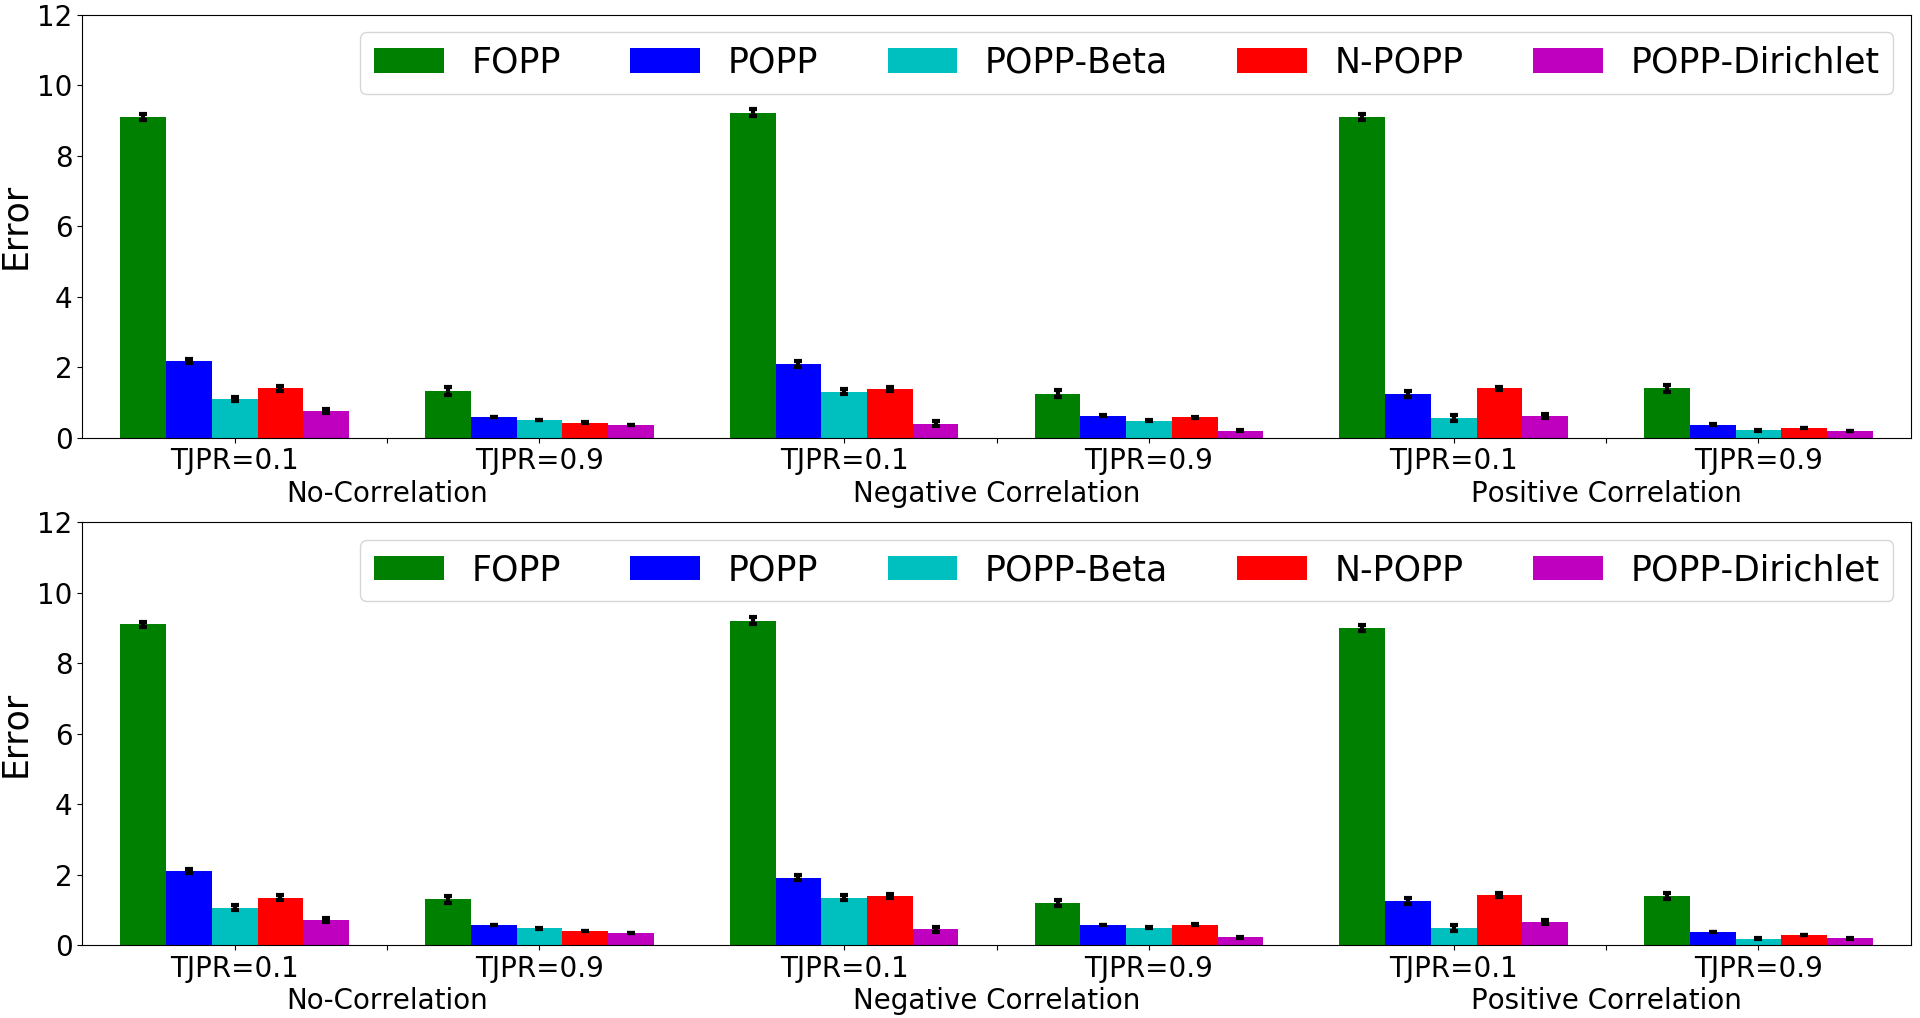
\includegraphics[width=0.5\textwidth]{./figures/tjpr_comparison_120.png}
    \caption{The RMSE of posterior estimates of $\lambda$ for the POPP and its variation models with 120 sample data used to build the (joint) sensor model with variation on $\mathcal{E^+}$. All models are compared to the FOPP model. Each trial consisted of a stream of $\protect\vec{s_1} \ldots \protect\vec{s_{144}}$ samples to update $P(\lambda ; \protect\vec{s_i})$. Accuracies of MAP estimates are shown in the top panel, accuracies of expectation of the posterior in the bottom panel. Each data point is an average of 30 trials. Standard errors are shown.} 
	\label{fig:tjpr_comparison_120}
\end{figure}

\begin{figure}[t!]
	\centering
	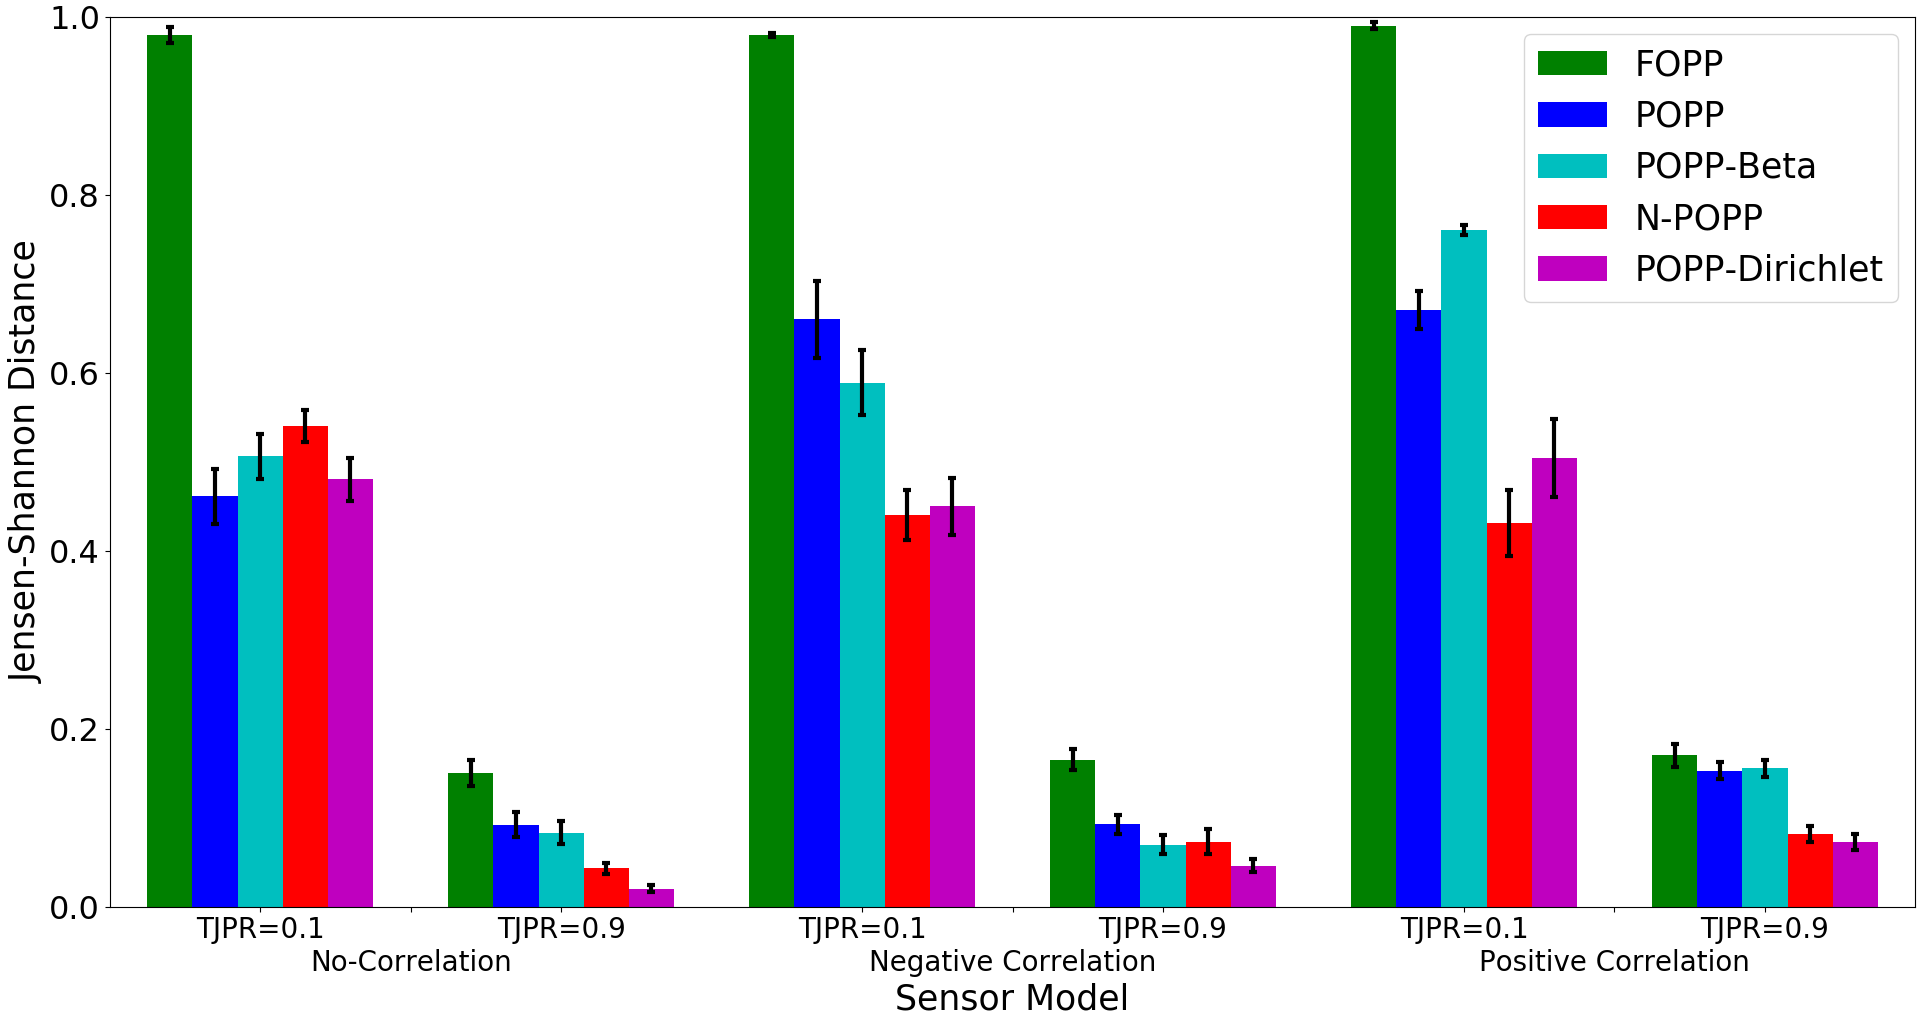
\includegraphics[width=0.5\textwidth]{./figures/tjpr_comparison_120_kl.png}
	\caption{The Jensen-Shannon distance of posterior estimates of $\lambda$ for the POPP and its variation models with 120 sample data used to build the (joint) sensor model with variation on $\mathcal{E^+}$. All models are compared to the FOPP model. Each trial consisted of a stream of $\protect\vec{s_1} \ldots \protect\vec{s_{144}}$ samples to update $P_G(\lambda \mid \protect\vec{s_i})$. Each data point is an average of 30 trials. Standard errors are shown.} 
	\label{fig:tjpr_comparison_120_kl}
\end{figure}

Different correlations between two sensors were tested: positive correlation, negative correlation, and no correlation. These correlations are designed to show the benefit of the C-POPP and POPP-Dirichlet models over the POPP and  POPP-Beta models (which assume sensors to be uncorrelated). For each correlation type, a further variation to different levels of sensor unreliability was considered. The true joint positive rate $\mathcal{E^+}$ (TJPR) and the true joint negative rate $\mathcal{E^-}$ (TJNR) were set as basis for varying sensor unreliability. For example, having TJPR configured with $P_{jnt}(d_{1k}=1, d_{2k}=1 ; e_k=1) = 0.1, P_{jnt}(d_{1k}=0, d_{2k}=0 ; e_k=1) = 0.9$ means that the true positive rate (TPR) for each sensor $j$ is $\textrm{\textit{tpr}}_j = P_j(d_k = 1; e_k=1) = 0.1$.

First, two variations were made to the true joint positive rate $\mathcal{E^+}$ (TJPR), while fixing the true joint negative rate $\mathcal{E^-}$ (TJNR) on each type of correlation. This includes:
\begin{itemize}
    \item $P_{jnt}(d_{1k}=1, d_{2k}=1 ; e_k=1) = 0.1, P_{jnt}(d_{1k}=0, d_{2k}=0 ; e_k=1) = 0.9$ ($\mathcal{E^+}$ with low positive correlation);
    \item $P_{jnt}(d_{1k}=1, d_{2k}=1 ; e_k=1) = 0.9, P_{jnt}(d_{1k}=0, d_{2k}=0 ; e_k=1) = 0.1$ ($\mathcal{E^+}$ with high positive correlation);
    \item $P_{jnt}(d_{1k}=1, d_{2k}=0 ; e_k=1) = 0.05, P_{jnt}(d_{1k}=0, d_{2k}=1 ; e_k=1) = 0.05, P_{jnt}(d_{1k}=0, d_{2k}=0 ; e_k=1) = 0.9$ ($\mathcal{E^+}$ with low negative correlation);
    \item $P_{jnt}(d_{1k}=1, d_{2k}=0 ; e_k=1) = 0.45, P_{jnt}(d_{1k}=0, d_{2k}=1 ; e_k=1) = 0.45, P_{jnt}(d_{1k}=0, d_{2k}=0 ; e_k=1) = 0.1$ ($\mathcal{E^+}$ with high negative correlation);
    \item $P_{jnt}(d_{1k}=1, d_{2k}=0 ; e_k=1) = 0.033, P_{jnt}(d_{1k}=0, d_{2k}=1 ; e_k=1) = 0.033, P_{jnt}(d_{1k}=1, d_{2k}=1 ; e_k=1) = 0.033, P_{jnt}(d_{1k}=0, d_{2k}=0 ; e_k=1) = 0.901$ ($\mathcal{E^+}$ with no correlation -- Similar to a sensor model with TPR = 0.066);
    \item $P_{jnt}(d_{1k}=1, d_{2k}=0 ; e_k=1) = 0.3, P_{jnt}(d_{1k}=0, d_{2k}=1 ; e_k=1) = 0.3, P_{jnt}(d_{1k}=1, d_{2k}=1 ; e_k=1) = 0.3, P_{jnt}(d_{1k}=0, d_{2k}=0 ; e_k=1) = 0.1$ ($\mathcal{E^+}$ with no correlation -- Similar to a sensor model with TPR = 0.6).
\end{itemize}

Second, two variations to the true joint negative rate $\mathcal{E^-}$ (TJNR), while fixing the true joint positive rate $\mathcal{E^+}$ (TJPR) on each type of correlation. This includes: 
\begin{itemize}
	\item $P_{jnt}(d_{1k}=1, d_{2k}=1 ; e_k=0) = 0.1, P_{jnt}(d_{1k}=0, d_{2k}=0 ; e_k=0) = 0.9$ ($\mathcal{E^-}$ with low positive correlation);
	\item $P_{jnt}(d_{1k}=1, d_{2k}=1 ; e_k=0) = 0.9, P_{jnt}(d_{1k}=0, d_{2k}=0 ; e_k=0) = 0.1$ ($\mathcal{E^-}$ with high positive correlation);
	\item $P_{jnt}(d_{1k}=1, d_{2k}=0 ; e_k=0) = 0.05, P_{jnt}(d_{1k}=0, d_{2k}=1 ; e_k=0) = 0.05, P_{jnt}(d_{1k}=0, d_{2k}=0 ; e_k=0) = 0.9$ ($\mathcal{E^-}$ with low negative correlation);
	\item $P_{jnt}(d_{1k}=1, d_{2k}=0 ; e_k=0) = 0.45, P_{jnt}(d_{1k}=0, d_{2k}=1 ; e_k=0) = 0.45, P_{jnt}(d_{1k}=0, d_{2k}=0 ; e_k=0) = 0.1$ ($\mathcal{E^-}$ with high negative correlation);
	\item $P_{jnt}(d_{1k}=1, d_{2k}=0 ; e_k=0) = 0.033, P_{jnt}(d_{1k}=0, d_{2k}=1 ; e_k=0) = 0.033, P_{jnt}(d_{1k}=1, d_{2k}=1 ; e_k=0) = 0.033, P_{jnt}(d_{1k}=0, d_{2k}=0 ; e_k=1) = 0.901$ ($\mathcal{E^-}$ with no correlation -- Similar to a sensor model with low TNR);
	\item $P_{jnt}(d_{1k}=1, d_{2k}=0 ; e_k=0) = 0.3, P_{jnt}(d_{1k}=0, d_{2k}=1 ; e_k=0) = 0.3, P_{jnt}(d_{1k}=1, d_{2k}=1 ; e_k=0) = 0.3, P_{jnt}(d_{1k}=0, d_{2k}=0 ; e_k=1) = 0.1$ ($\mathcal{E^-}$ with no correlation -- Similar to a sensor model with moderate TNR).
\end{itemize}

The performance of all POPP models were assessed by comparing how accurate each model is in estimating the true $\lambda'$. Two options were used to do this: (1) a distance metric method using the RMSE of the expectation (mean) and the MAP hypothesis (mode) of each model posterior distribution over $\lambda$ to the true $\lambda'$ and (2) a free-distance metric method using the Jensen-Shannon distance between the posterior distribution $P(\lambda ; \vec{s_i})$ and the distribution of the true $\lambda'$. 

\begin{figure}[t!]
	\centering
	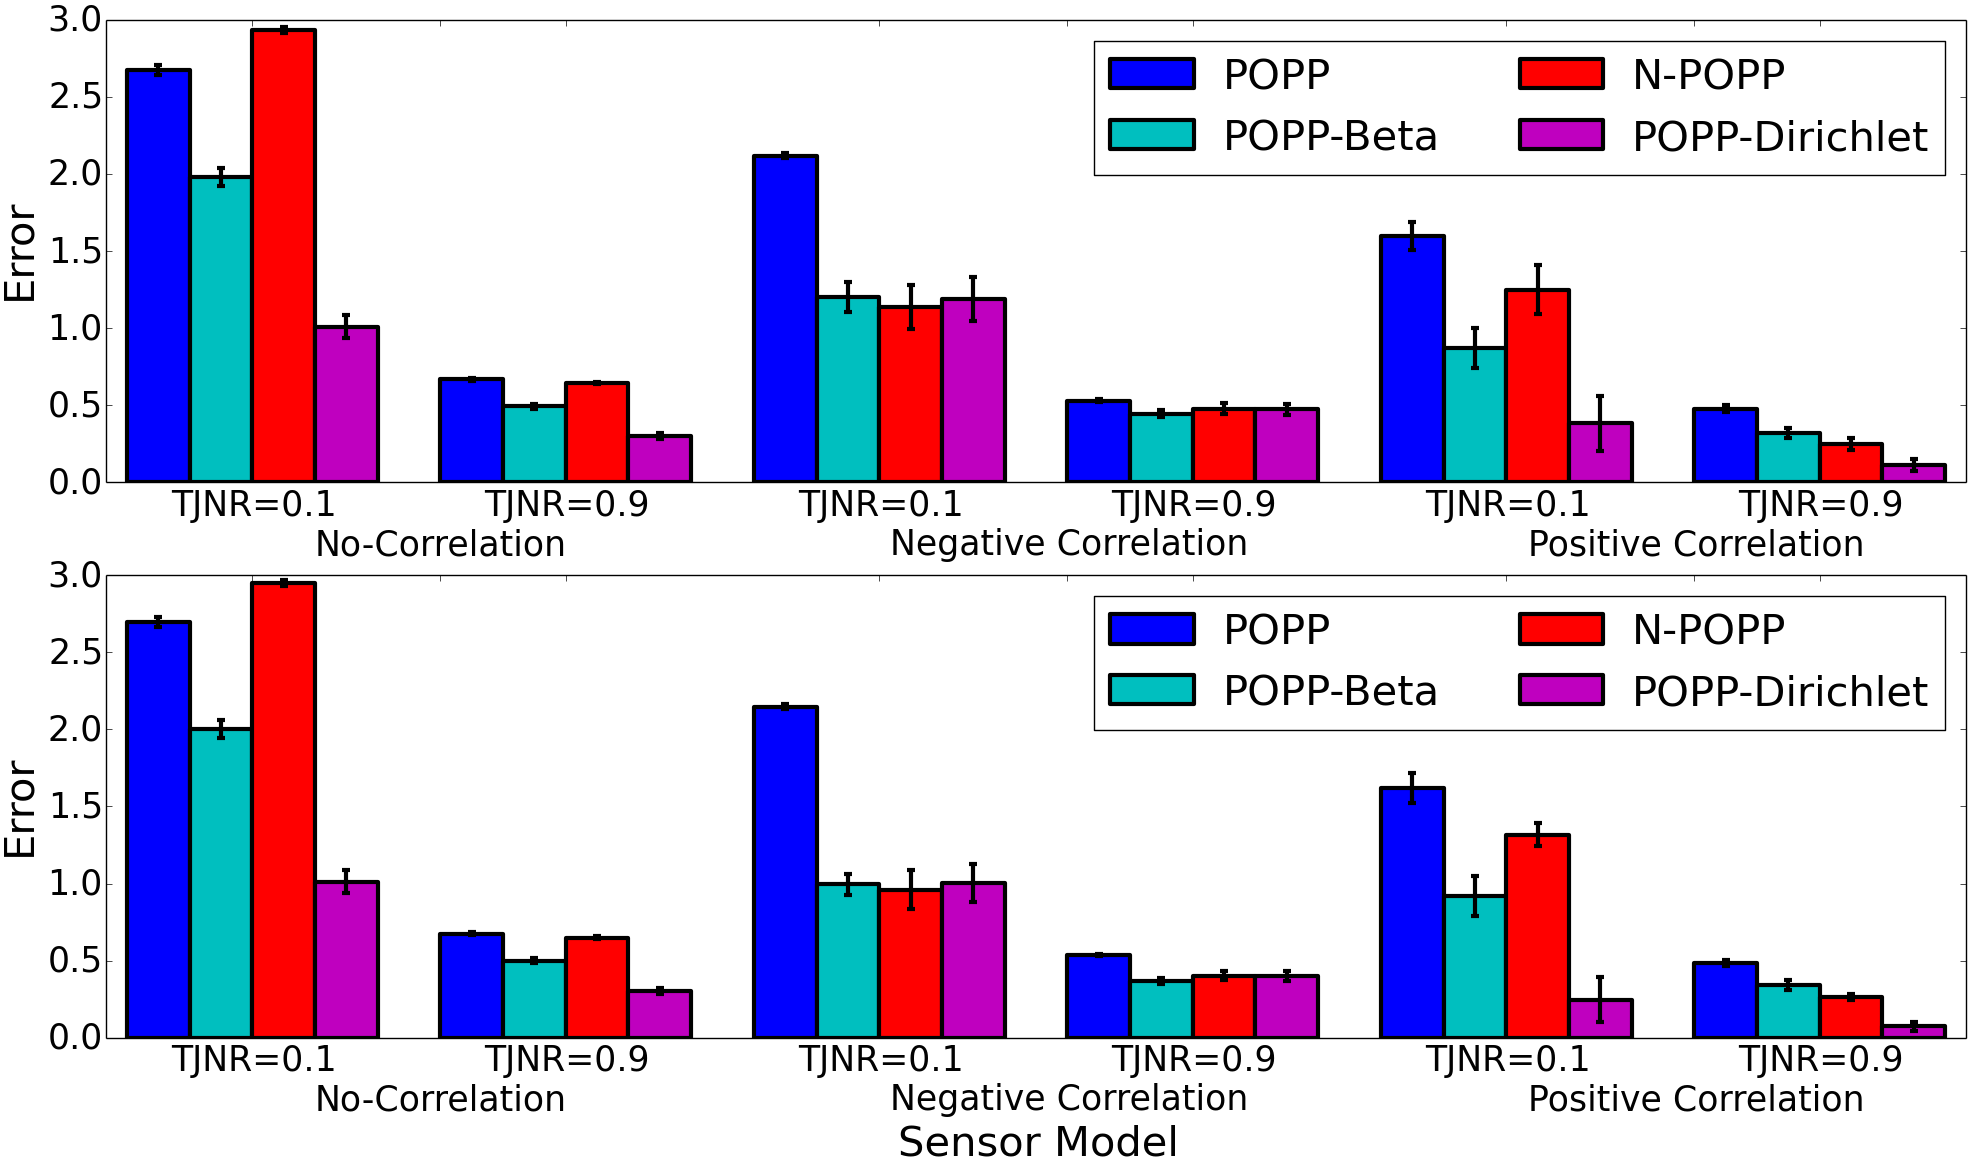
\includegraphics[width=0.5\textwidth]{./figures/tjnr_comparison_120.png}
    \caption{The RMSE of posterior estimates of $\lambda$ for the POPP and its variation models with 120 sample data used to build the (joint) sensor model with variation in $\mathcal{E^-}$. All models are compared to the FOPP model. Each trial consisted of a stream of $\protect\vec{s_1} \ldots \protect\vec{s_{144}}$ samples to update $P(\lambda ; \protect\vec{s_i})$. Accuracies of MAP estimates are  in the top panel, accuracies of the expectation of the posterior in the bottom panel. Each data point is an average of 30 trials. Standard errors are shown.} 
	\label{fig:tjnr_comparison_120}
\end{figure}

\begin{figure}[t!]
	\centering
	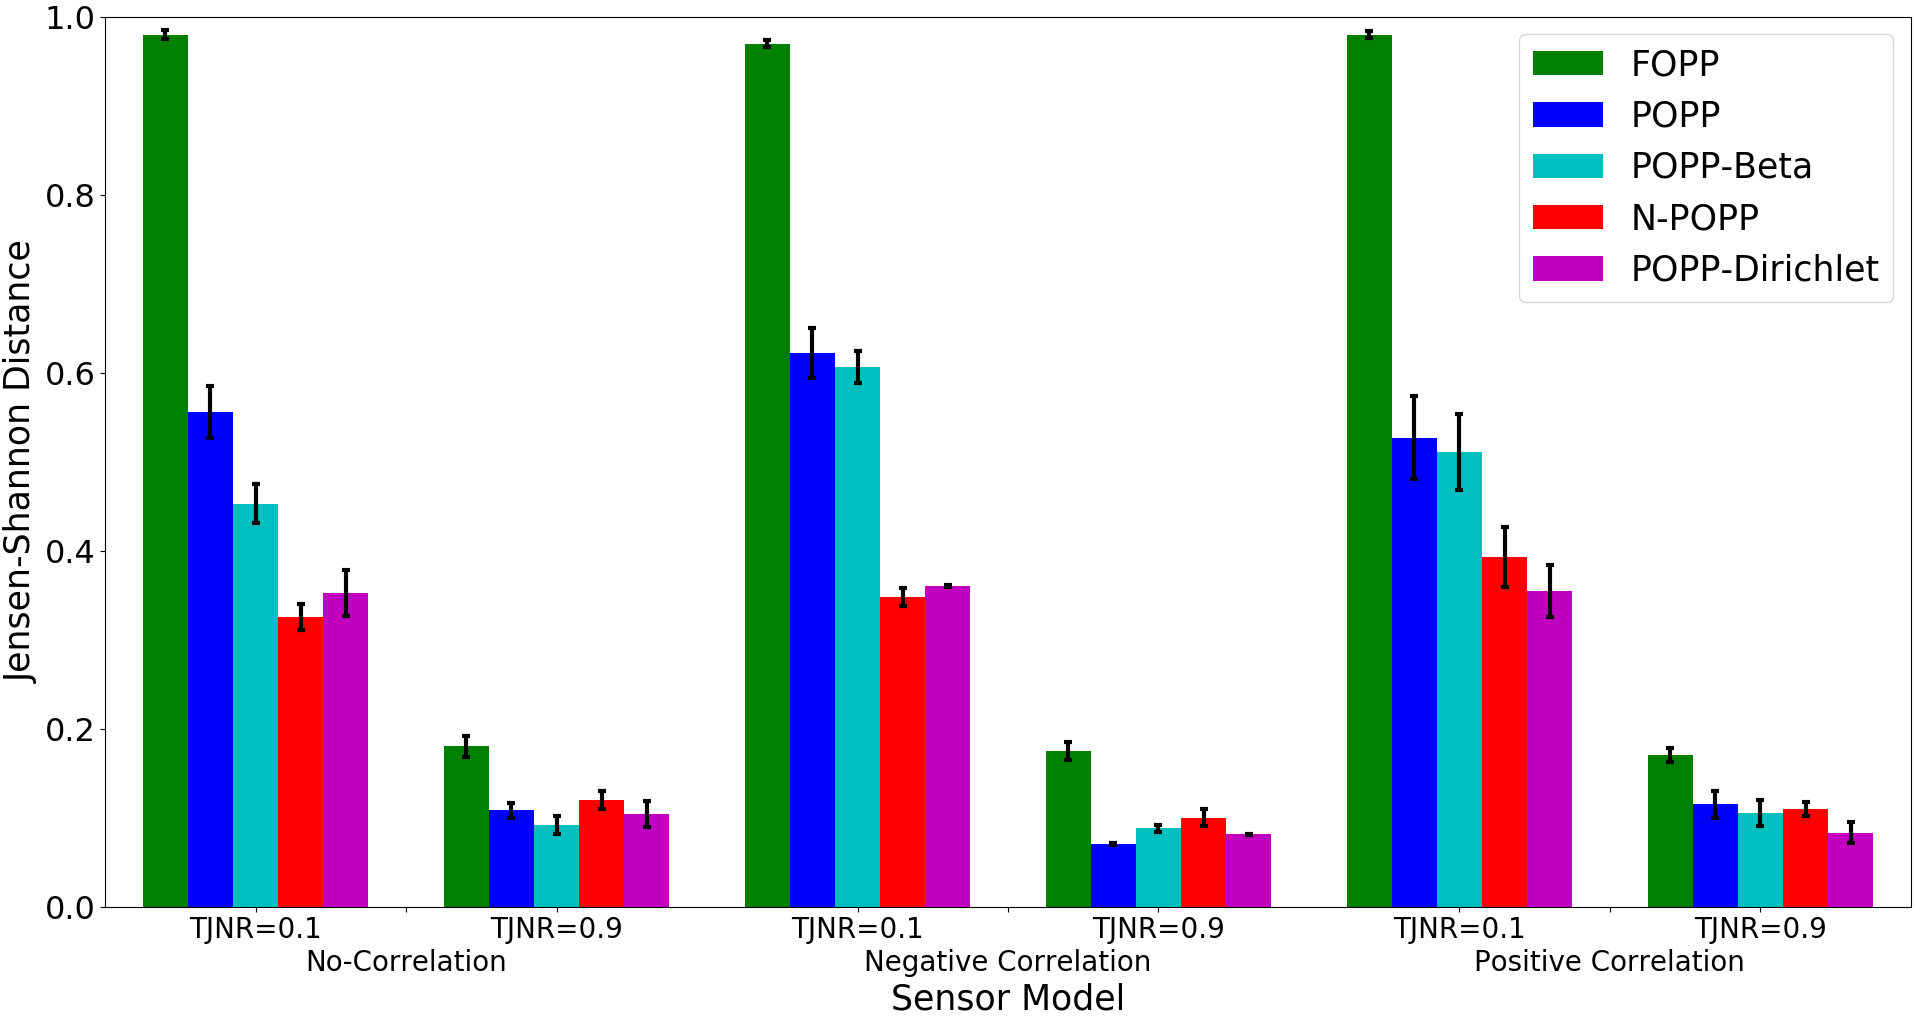
\includegraphics[width=0.5\textwidth]{./figures/tjnr_comparison_120_kl.png}
	\caption{The Jensen-Shannon distance of posterior estimates of $\lambda$ for the POPP and its variation models with 120 sample data used to build the (joint) sensor model with variation on $\mathcal{E^-}$. All models are compared to the FOPP model. Each trial consisted of a stream of $\protect\vec{s_1} \ldots \protect\vec{s_{144}}$ samples to update $P_G(\lambda \mid \protect\vec{s_i})$. Each data point is an average of 30 trials. Standard errors are shown.} 
	\label{fig:tjnr_comparison_120_kl}
\end{figure}

Figure \ref{fig:tjpr_comparison_120} and \ref{fig:tjpr_comparison_120_kl} show the accuracy of all POPP models on the variation of true joint positive rate, whereas figure \ref{fig:tjnr_comparison_120} and \ref{fig:tjnr_comparison_120_kl} show the accuracy on the variation of the true joint negative rate. From these figures, the POPP-Beta and POPP-Dirichlet show a better accuracy than the POPP and the C-POPP. The C-POPP and the POPP-Dirichlet which utilize correlation among sensors to estimate the arrival rate $\lambda'$ tend to be more accurate than the standard POPP and POPP-Beta.
In general, the POPP-Dirichlet tends to be more accurate than any other POPP model thanks to its ability to model correlation among sensors and to model how confident it is with its sensor model.

%!TEX root = ../bare_jrnl.tex

\section{Evaluation on Aggregate Human Occupancy Behaviour Dataset}
\label{sec:evareal}

We now investigate the performance of the POPP model and its extensions on a real world dataset\footnote{The dataset can be downloaded from \url{https://github.com/ferdianjovan/spectral_popp}}.
% 
The dataset was gathered from an office building in which a mobile robot~\cite{hawes2016strands} counted the number of people in different regions whilst patrolling (see Figure~\ref{fig:map_popp_independent_test} for the map of the building). The dataset contains time series  counts from three different automated person detectors~\cite{dondrup2015real}. These use laser, depth camera and RGB information. We refer to these detectors respectively as the leg detector (LD), upper body detector (UBD), and change detector (CD). Each of these detectors acts as one sensor. Each returns a sensed count of the number of people it detected in each 10 minute interval during the day. These detectors are unreliable, as can be seen from Figure~\ref{fig:single_sensor_rate_transformation}, which shows examples of correct and incorrect detections.

\begin{figure}[t]
	\centering
	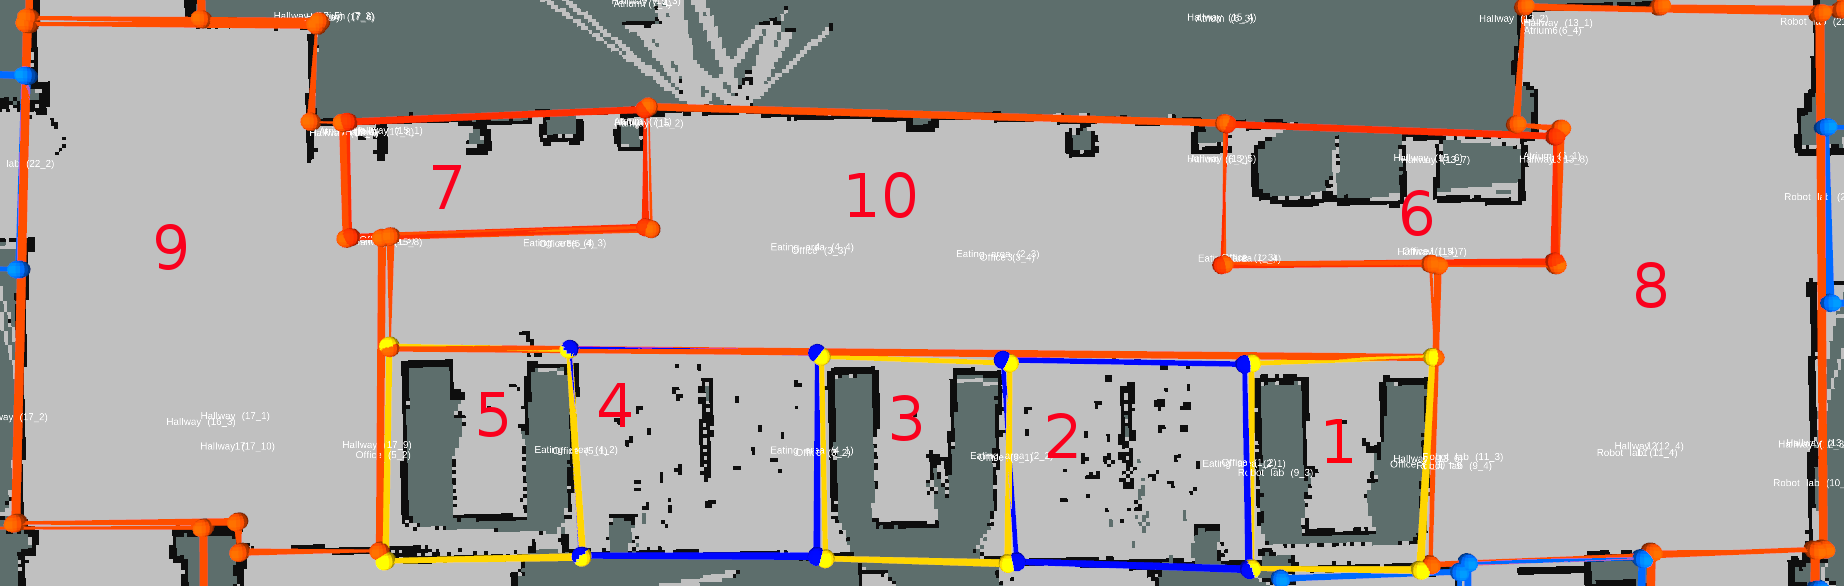
\includegraphics[width=0.95\columnwidth]{./figures/map_popp.png}
	\caption{The office building in which the robot gathered data. Areas are bounded by imaginary lines.}
	\label{fig:map_popp_independent_test}
\end{figure}

\begin{figure}[t]
	\centering
	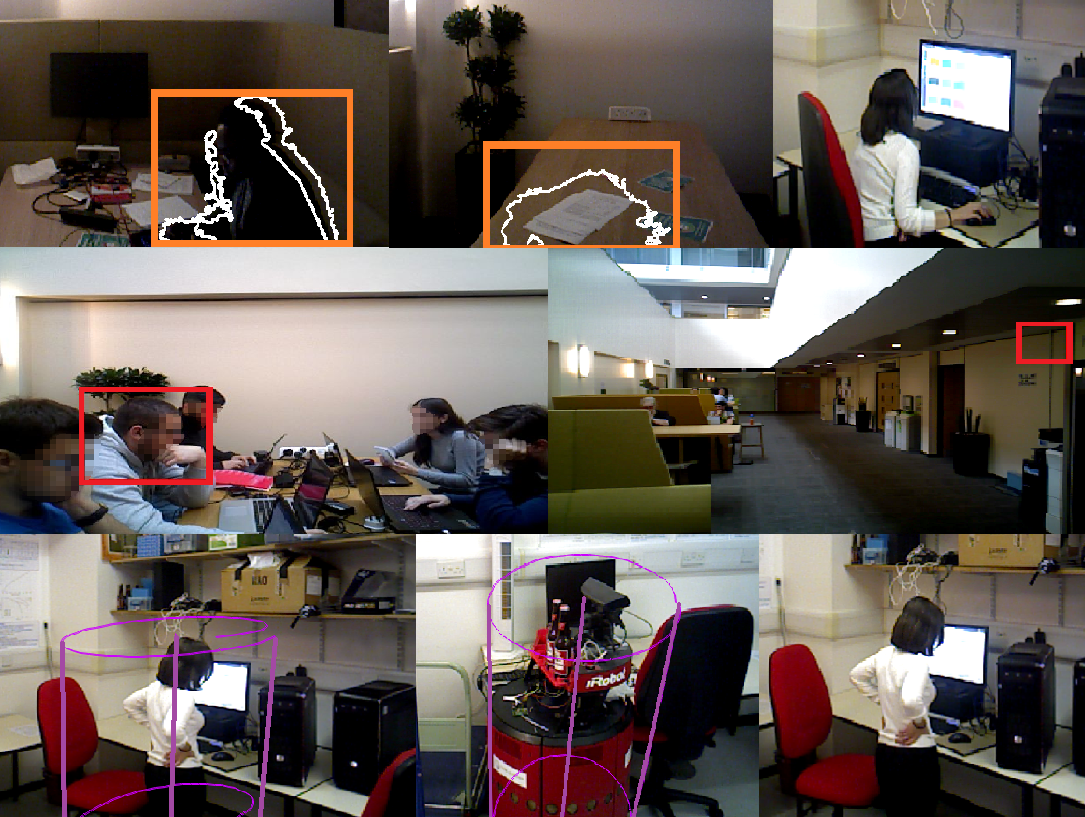
\includegraphics[width=0.95\columnwidth]{./figures/sensor_images.png}
	\caption{Correct and incorrect detections, and non-detections, from different regions in the environment for each sensor. Top row: change detector. Middle row: upper body detector. Bottom row: leg detector. Detections are marked with 2D or 3D bounding boxes. A bounding box containing a person is a correct detection (true positive). One without a person is an incorrect detection (false positive). A person without a bounding box is a missed detection (false negative).}
	\label{fig:single_sensor_rate_transformation}
\end{figure}

By comparing the ground truth with the detections made by sensors, we compute a sensor model for each region. An average of the sensor models across all regions can be seen in Table \ref{table:sensor_model_popp_beta}. Although the robot operated for 24 hours day, the sensor models were built using only the data collected from 10am to 8pm, since there were few detections outside these times. From a 69 day deployment of the mobile robot, we obtained 48 days of usable observations. We specified a time interval for each Poisson distribution of 10 minutes, and recorded both the true counts and the detections made by each sensor in each interval. We assumed the underlying process in each region to be a periodic Poisson process in which there is a one-day periodicity, i.e. $\lambda(t) = \lambda(t + \Delta)$ with $\Delta = 24 * 60$ (minutes). This means that the expected number of people each day at a particular time is expected to be the same across the 48 days of observations. We estimated the true parameter $\lambda'(t)$ of the Poisson distribution at $t$ by running a FOPP model on the true counts within each interval. We use this estimate of $\lambda'(t)$ from the true counts as the target which the POPP models must estimate from the sensed counts.

The different POPP approaches rely on sensor models that must be calculated from a confusion matrix relating true counts to the sensed counts from the different sensors. To separate the training and testing data we performed four fold cross-validation with data splits being on whole days, i.e., we used 12 days of data as a training set for a sensor model and then used the remaining 36 days of data as a test set on which to test the inferences made by each model from the sensor counts.

\begin{table}[t]
	\centering
	\caption{Averaged sensor models across all areas trained from 48 days of data.}
	\label{table:sensor_model_popp_beta}
	\begin{tabular}{lccc}
		\noalign{\hrule height 1.1pt}\noalign{\smallskip}
		Sensor & True Positive & True Negative \\
		\noalign{\smallskip}\hline\noalign{\smallskip}
		Leg Detector & 0.387 & 0.951 \\
		Upper Body Detector & 0.356 & 0.882 \\
		Change Detector & 0.731 & 0.900 \\ 
		\noalign{\hrule height 1.1pt}\noalign{\smallskip}
	\end{tabular}
\end{table}

For the 36 days of test data, the different models each made predictions of the $\lambda(t)$ parameter of the Poisson. Given this, we recorded (1) the RMSE between the MAP hypothesis of each model posterior distribution over $\lambda(t)$ and the true $\lambda'(t)$ and (2) the Jensen-Shannon distance between the posterior distribution $P(\lambda(t) \mid \mathbf{s_i})$ and the distribution of the true $\lambda'(t)$. Using these metrics, we compared the performance of all POPP models (estimated using the switching filter described in~\ref{sec:estimators}) to the Bayes' filter arising from the FOPP model. The FOPP model is a single sensor model and was estimated from the change detector counts since this was the most reliable detector among the three available (as shown in Table~\ref{table:sensor_model_popp_beta}). 

Figures \ref{fig:fopp_popp_popb_npop_popd_rmse_evo} and \ref{fig:fopp_popp_popb_npop_popd_kl_evo} show the accuracy comparison between all POPP models and the standard FOPP model over time. It can be seen that all models become more accurate as the days pass. All POPP models show more accuracy over the standard FOPP model. The $\lambda(t)$ estimate produced by the POPP-Dirichlet model is more accurate than the ones produced by the standard POPP model and the POPP-Beta model. However, the POPP-Dirichlet estimate is not always more accurate than the one produced by the C-POPP model. 

As the POPP-Dirichlet model is more conservative in estimating the parameter $\lambda(t)$ than the C-POPP model, the estimate moves more slowly towards the true $\lambda'(t)$. This is seen in Figure~\ref{fig:fopp_popp_popb_npop_popd_kl_evo}.
By the third day, the POPP-Dirichlet model outperformed the POPP, POPP-Beta, and C-POPP models in terms of accuracy. However, the accuracy gap between the C-POPP model and the POPP-Dirichlet model becomes smaller over time. By the 36th day the C-POPP model outperforms the POPP-Dirichlet only by a small margin.

\begin{figure}[t!]
	\centering
	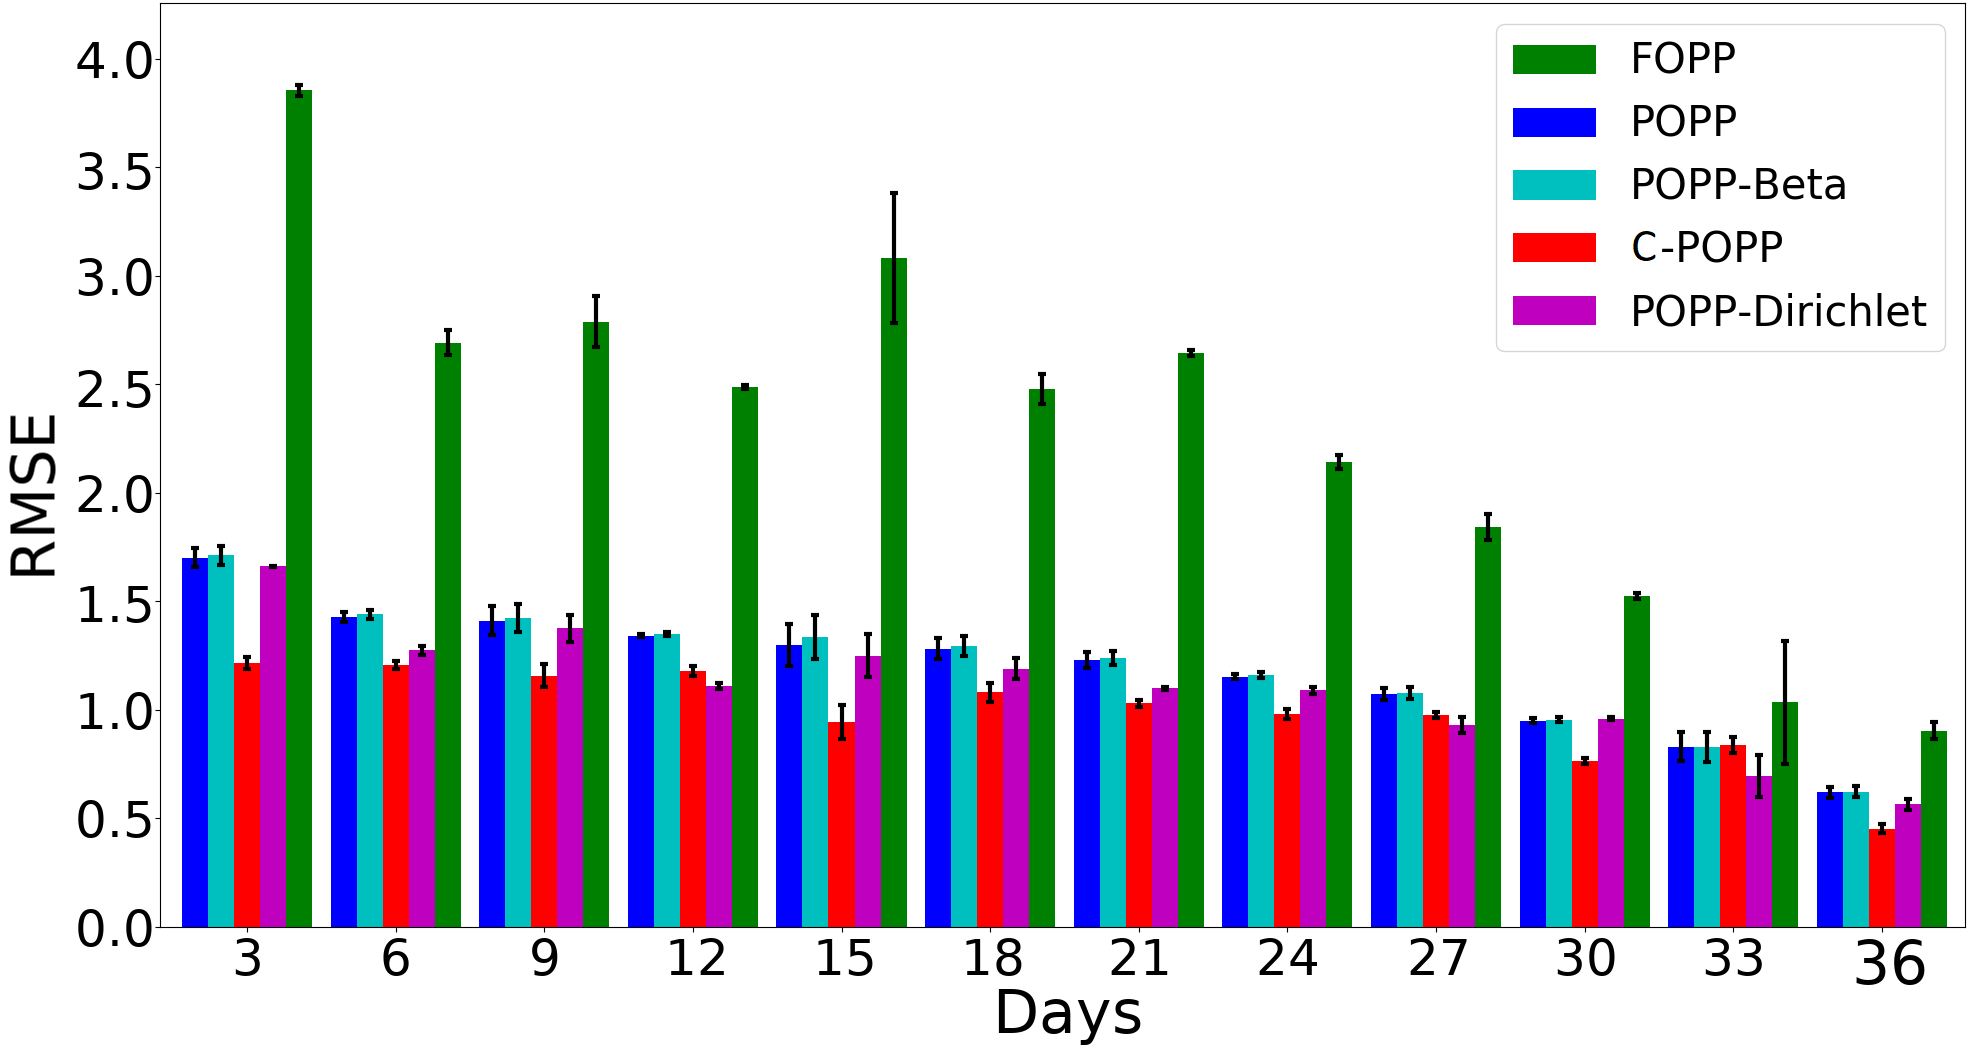
\includegraphics[width=0.95\columnwidth]{./figures/fopp_popp_popb_npop_popd_rmse_evo.png}
	\caption{The RMSE evolution of periodic Poisson processes with POPP, POPP-Beta, C-POPP, POPP-Dirichlet and FOPP filters from day 3 to day 36, averaged across all regions. Standard error is shown.}
	\label{fig:fopp_popp_popb_npop_popd_rmse_evo}
\end{figure}

\begin{figure}[t!]
	\centering
	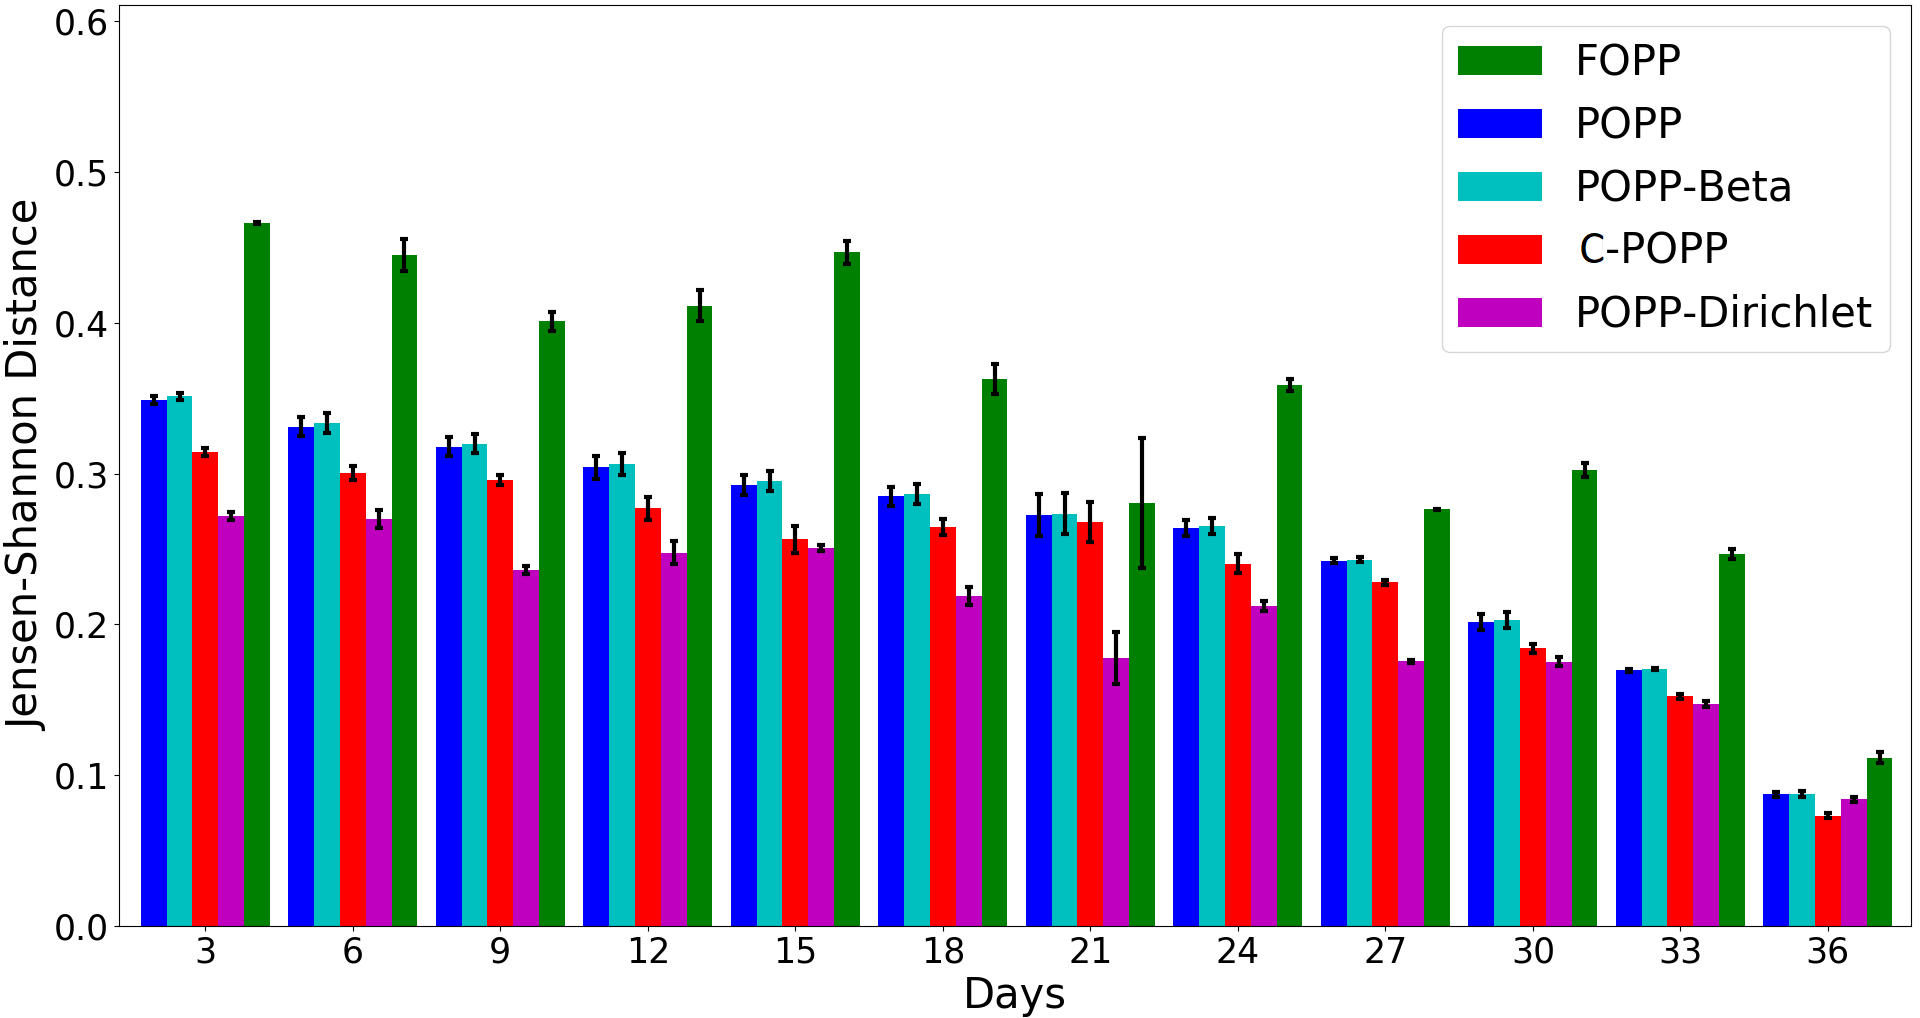
\includegraphics[width=0.95\columnwidth]{./figures/fopp_popp_popb_npop_popd_kl_evo.png}
	\caption{The Jensen-Shannon distance evolution of the FOPP, the POPP, the POPP-Beta, the C-POPP, and the POPP-Dirichlet filters in periodic Poisson processes from day 3 to day 36 in a 3-day interval, averaged across all regions. Standard error is shown.}
	\label{fig:fopp_popp_popb_npop_popd_kl_evo}
\end{figure}

\begin{figure}[t!]
	\centering
	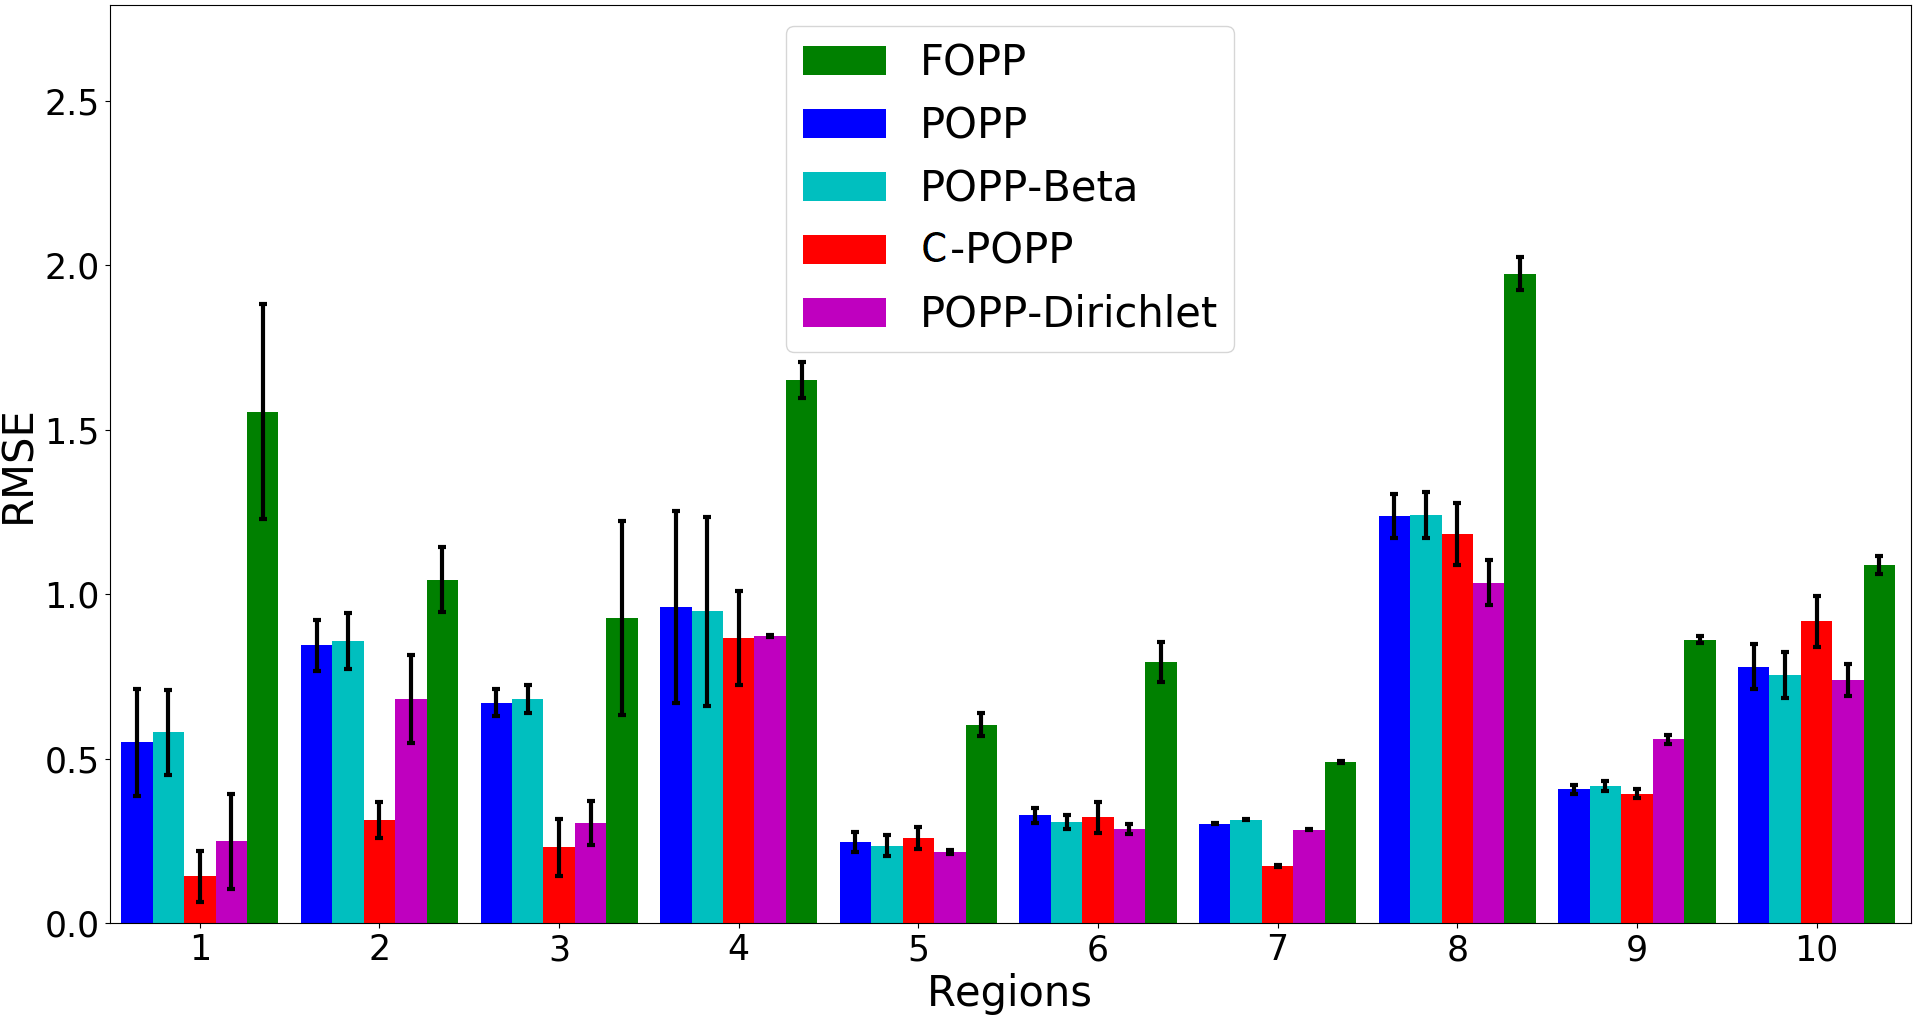
\includegraphics[width=0.95\columnwidth]{./figures/fopp_popp_popb_npop_popd_rmse.png}
	\caption{The RMSE of the FOPP, POPP, POPP-Beta, C-POPP, and POPP-Dirichlet filters across regions. The RMSE(s) are taken at the 36th day. Standard error is shown.}
	\label{fig:fopp_popp_popb_npop_popd_rmse}
\end{figure}

\begin{figure}[t!]
	\centering
	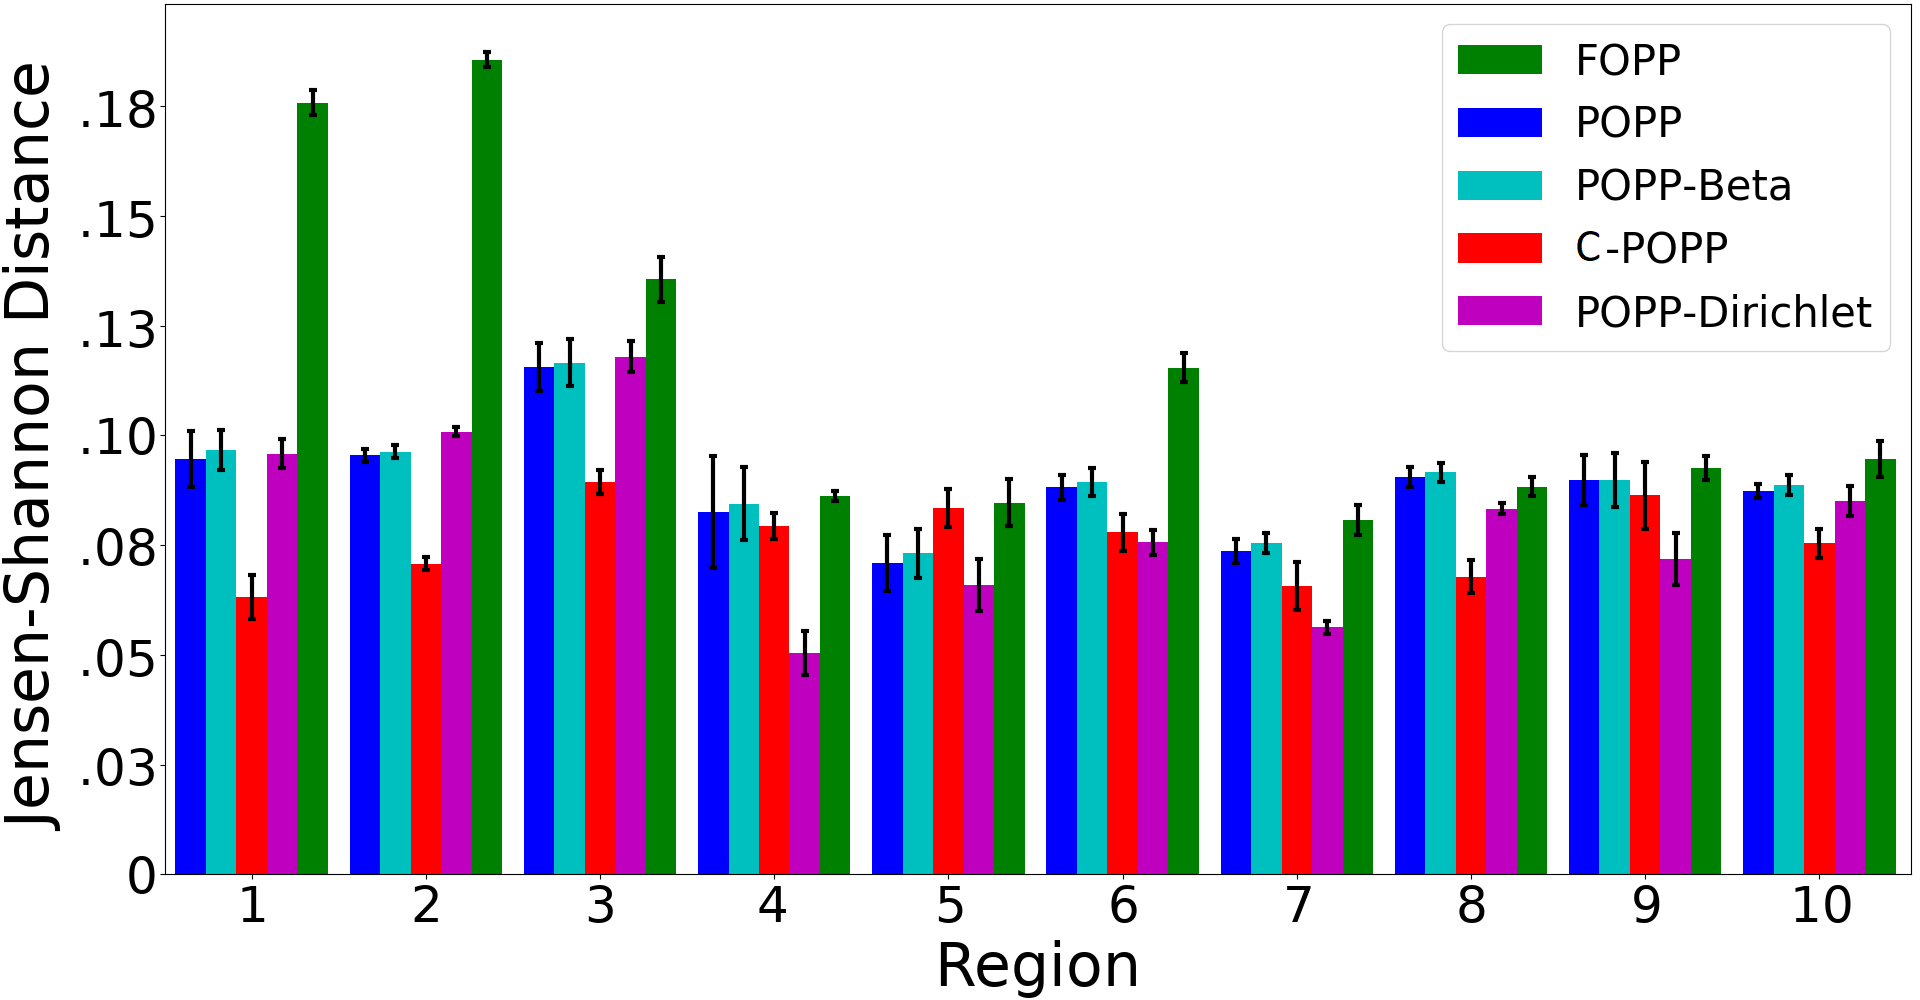
\includegraphics[width=0.95\columnwidth]{./figures/fopp_popp_popb_npop_popd_kl.png}
	\caption{The Jensen-Shannon of the FOPP, POPP, POPP-Beta, C-POPP, and POPP-Dirichlet filters across regions. The Jensen-Shannon value(s) are taken at the 36th day. Standard error is shown.}
	\label{fig:fopp_popp_popb_npop_popd_kl}
\end{figure}


Figure \ref{fig:fopp_popp_popb_npop_popd_rmse} and \ref{fig:fopp_popp_popb_npop_popd_kl} show the RMSE and Jensen-Shannon comparison between all POPP models and the FOPP across different regions by the end of the 36th day. It can be seen that the POPP-Dirichlet and the C-POPP once again outperformed the other models. Some regions such as 1, 2, and 3 have much more data than other regions. Since this  provides  more data to create the sensor models than other regions, the point-estimate joint sensor model for the C-POPP filter can be more accurately estimated for these regions. Unlike C-POPP filter, the POPP-Dirichlet estimates the joint sensor model as a distribution. As a result, the C-POPP filter estimates for these regions become more accurate than the POPP-Dirichlet. 

%Similar to the C-POPP model, the POPP-Dirichlet model is able to cope and overcome the problems with limited sample data both for building the joint sensor model and estimating the $\lambda(t_i, t_j)$. In many regions, the POPP-Dirichlet managed to show better estimates as well as more similar distributions than the POPP, the POPP-Beta, and the FOPP models. However, the POPP-Dirichlet filter falls behind both in accuracy (RMSE) and distribution similarity compared to the C-POPP model. This is attributed to the POPP-Dirichlet conservative way in estimating the parameter $\lambda(t_i, t_j)$ compared to the C-POPP model.
%!TEX root = ../bare_jrnl.tex

\section{Exploration on Human Occupancy Behaviour}
\label{sec:exploration}

So far, the paper has focused on Bayesian methods for inferring a belief state about the spatio-temporal patterns of human occupancy from unreliable sensors. Given such a belief state a robot may plan how to actively explore to acquire new information or to complete a task~\cite{hanheide2017robot}. In this section, we use the resulting predictions to drive robotic \emph{exploration} to detect human activities at an increasing rate. In particular, the robot should determine an exploration policy which is a function of its belief and which will, over time, take it to regions with the highest aggregate level of human activity.

\subsection*{Exploration Models}

The problem addressed is how the robot should plan to explore so as to maximise the observed number of human activities over time. This an instance of an \emph{exploration-exploitation} problem.
% 
Exploration-exploitation problems arise when an agent, in this scenario a mobile robot, does not fully understand the process it is trying to control. At any time, the agent can choose to explore or to exploit its model of the process.
Exploration allows the agent to better understand the process by gathering more data, leading to a better action later on, but sacrificing short-term reward.
Exploitation allows the agent to  leverage what it already understands about the process to gain reward immediately, but risks following a policy that might be suboptimal. 
% 
Our decision problem is a choice between which regions to visit next, as each region will offer the robot different exploration-exploitation opportunities.

% In each time the robot has a choice between many actions, each of which both explores and exploits a certain place, but to varying degrees. As its goal is to maximise the reward gathered–as in getting as much data on human activities (by seeing as many humans) as possible–given its limited operational life, it is preferable to have a policy that is as near optimal as possible.

While exploration-exploitation problems in reinforcement learning are typically intractable, there are well known approximate approaches that are quick to compute~\cite{wyatt1998exploration, 1413255, AUDIBERT20091876}. One such approach is to use the upper bound of a probability distribution over the quantity being maximised. This causes the decision-making agent to exploit high-scoring, certain estimates, and explore highly uncertain estimates. In our robot exploration, for example, when the robot visits a place, it can be because the place either actually has high number of people (\textit{exploitation}) or potentially has high number of people (\textit{exploration}). In our case we use an upper bound on the arrival rate ($\lambda$) of a Poisson process ($\lambda_{UB}$) to choose the region for the robot to visit next. The upper bound of the probability interval of the arrival rate of a Poisson process is calculated as follows:

\begin{equation}
	\label{eq:upper_bound_exploration}
	\begin{tabular}{r@{ = }l}
	$\lambda_{UB}(t_i, t_j)$ & $\displaystyle \int_{t_i}^{t_j} CDF^{-1}(\% = 0.95 \mid \alpha_t, \beta_t)~dt$\\ [1ex]
	\end{tabular}
\end{equation}

\noindent with $\lambda_{UB}(t_i, t_j)$ as the upper bound of $\lambda$ within time $t_i$ and $t_j$, $i, j \in \{1, \ldots, \Delta\}$, and $CDF^{-1}$ as the inverse of the cumulative density function of a Gamma distribution. Given the upper bounds $\lambda^{r}_{UB}(t_i, t_j)$ for each region $r$ from the set of all regions $R$, the region to be visited between time $t_i$ and $t_j$ is chosen by:

\begin{equation}
\label{eq:choosing_place}
\underset{r \in \mathcal R}{\arg\max}~\lambda^{r}_{UB}(t_i, t_j)
\end{equation}
\noindent Figure~\ref{fig:map_vs_ub} depicts a comparison between the MAP hypothesis estimate and the upper bound estimate of a Poisson process.

\begin{figure}[t!]
	\centering
	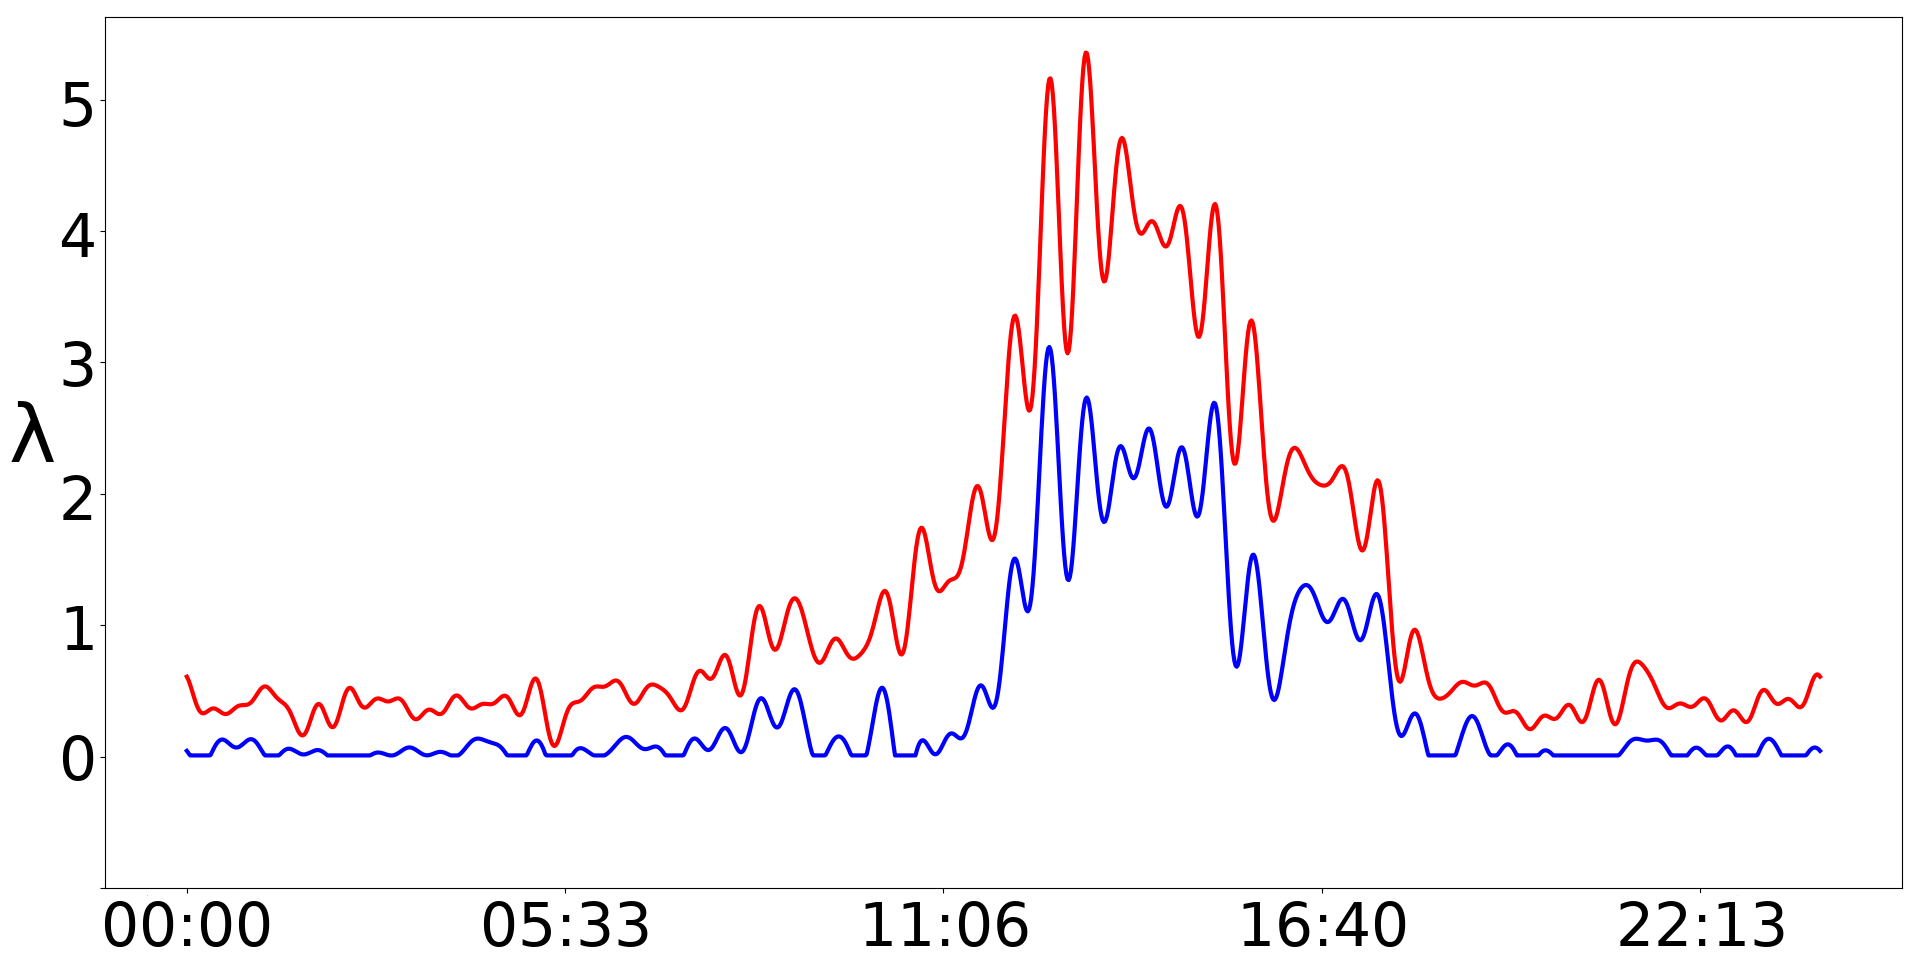
\includegraphics[width=0.5\textwidth]{./figures/map_vs_ub.png}
	\caption{A spectral Poisson process of region 9 (see Figure \ref{fig:map_popp_independent_test}) represented by its MAP hypothesis (blue line) and its upper bound of the probability interval (red line).}
	\label{fig:map_vs_ub}
\end{figure}


To tie the estimate of a particular Poisson process over a time interval to data collected previously, as in Section~\ref{sec:evareal} we assume that human presence in each region follows a \emph{periodic} Poisson process with daily periodicity. This allows us to regularise, and fill missing data, across the point estimates of upper bounds using methods based on the Fourier transform.  This exploits assumptions and algorithms introduced in our prior work. In particular, the series of upper bounds $\lambda_{UB}(t_i, t_j)$ are encoded and extracted via spectral analysis with the $l$-AAM technique described in~\cite{jovan_iros16}. The plot in Fig.~\ref{fig:map_vs_ub} shows how a spectral Poisson process look like, i.e., the effects of the spectral processing on a periodic Poisson process. Algorithm 2 depicts the process of computing the upper bound of a Poisson process and applying spectral analysis to it. We use this approach with upper bounds produced by our previously presented estimators: FOPP, POPP, and POPP-Beta. 

\begin{figure}[t!]
	\begin{center}
		\begin{tabular*}{0.5\textwidth}{l @{\extracolsep{\fill}}}
			\hline
			\textbf{l-AAM} \textrm{\cite{jovan_iros16}} \\
			\hline
			\textbf{Input:} $x_1, \ldots, x_n$: input signal, \\
			\hspace{0.3cm} total: maximum total frequency \\
			\textbf{Output:} $\mathcal S$: a collection of $(s, p, f)$ \\
			\textbf{Procedure:}\\
			\hspace{0.3cm} 1. Init. k $\leftarrow$ 0 \\
			\hspace{0.3cm} // Get frequency $0$ with Discrete Fourier Transform \\
			\hspace{0.3cm} 2. $[s, p, f] \leftarrow DFT(x_1, \ldots, x_n)[0]$\\
			\hspace{0.3cm} 3. $\mathcal S[k] \leftarrow [s, p, f]$ \\
			\hspace{0.3cm} 4. Repeat until k $>$ total \\
			\hspace{0.7cm} $\bullet ~ k \leftarrow k + 1$ \\
			\hspace{0.7cm} // Get the frequency with the highest amplitude \\
			\hspace{0.7cm} $\bullet ~ [s, p, f] \leftarrow \argmax_s DFT(x_1, \ldots, x_n)$ \\
			\hspace{0.7cm} // Update $\mathcal S$ with frequency $f$ \\
			\hspace{0.7cm} $\bullet$ if $f \in \mathcal S$, $[s', p', f'] \leftarrow \mathcal S[k', f'=f]$ \\
			\hspace{2.5cm} $s \leftarrow s + s'$; $p \leftarrow p + p'$ \\ 
			\hspace{0.7cm} $\bullet$ $\mathcal S[k] \leftarrow [s, p, f]$ \\
			\hspace{0.7cm} // Create a cosine signal from $f$ \\
			\hspace{0.7cm} $\bullet ~ x'_1, \ldots, x'_n \leftarrow s * ~ cos(2 \pi * f + p)$ \\
			\hspace{0.7cm} // Subtract current $x_1, \ldots, x_n$ with the cosine signal \\
			\hspace{0.7cm} $\bullet ~ x_1, \ldots, x_n \leftarrow x_1, \ldots, x_n - x'_1, \ldots, x'_n$ \\
			\hline
		\end{tabular*}	
	\end{center}
\end{figure}

\begin{figure}[t!]
	\begin{center}
		\begin{tabular*}{0.5\textwidth}{l @{\extracolsep{\fill}}}
			\hline
			\textbf{Algorithm 2} \textit{Upper Bound} \\
			\hline
			\textbf{Input:} $(\alpha_1, \beta_1), \ldots, (\alpha_n, \beta_n)$: Poisson process \\
			\textbf{Output:} $\lambda^{ub}_1, \ldots, \lambda^{ub}_n$: upper bound \\
			\textbf{Procedure:}\\
			\hspace{0.3cm} 1. Init. k $\leftarrow$ 1, m $\leftarrow$ $\eta$ \\
			\hspace{0.3cm} 2. Repeat until k $>$ n \\
			\hspace{0.7cm} $\bullet ~ k \leftarrow k + 1$ \\
			\hspace{0.7cm} // Get the upper bound \\
			\hspace{0.7cm} $\bullet ~ \lambda_k \leftarrow CDF(0.95, \alpha_k, \beta_k)$ \\
			\hspace{0.3cm} // Transform $\lambda_1, \ldots, \lambda_n$ to with $l$-AAM \\
			\hspace{0.3cm} 3. $\mathcal S$ $\leftarrow$ \textbf{l-AAM}($\lambda_1, \ldots, \lambda_n$, m) \\
			\hspace{0.3cm} 5. Init. k $\leftarrow$ 0,  $\lambda^{ub}_1, \ldots, \lambda^{ub}_n \leftarrow (0, \ldots, 0)$ \\
			\hspace{0.3cm} 4. Repeat until k $>$ m \\
			\hspace{0.7cm} // Create a cosine signal from $\mathcal S[k]$ \\
			\hspace{0.7cm} $\bullet ~ [s, p, f] \leftarrow \mathcal S[k]$ \\
			\hspace{0.7cm} $\bullet ~ x_1, \ldots, x_n \leftarrow s * ~ cos(2 \pi * f + p)$ \\
			\hspace{0.7cm} // Add current $\lambda^{ub}_1, \ldots, \lambda^{ub}_n$ with the cosine signal \\
			\hspace{0.7cm} $\bullet ~ \lambda^{ub}_1, \ldots, \lambda^{ub}_n \leftarrow \lambda^{ub}_1, \ldots, \lambda^{ub}_n + x_1, \ldots, x_n$ \\
			\hline
		\end{tabular*}	
	\end{center}
\end{figure} 


\subsection*{Exploration Evaluation}

The dataset used in the previous section was collected by a mobile robot over 69 days of a real world trial. This robot was controlled by the exploration models described above. Due to hardware failures, sensor malfunctions and other external issues, only 48 days from the dataset were usable.

Three different exploration models were applied separately during three phases of the 69 days of the trial. All of these models used Eq.~\ref{eq:choosing_place} to create their exploration policies. For the first 27 day phase of the trial, the robot followed an exploration policy based on the FOPP model. This resulted in 18 days of data. From day 28 to day 47, the robot followed an exploration policy according to the POPP model. This resulted in 15 days of data. Finally, from day 48 onwards, the robot followed an exploration policy according to the POPP-Beta model. This also resulted in 15 days of data. 
% 
Such that all three models can be compared equally, in the following we also constrain the data available for for the FOPP model to the first 15 of its 18 days.
% 
% From this 18 days of data, the last 3 days were used to train the sensor model needed for both the POPP and the POPP-Beta models.
%For this comparison, the last 3 days which are part of the 18 days worth of data collected by following the FOPP exploration model are included in the POPP and the POPP-Beta exploration models. This is necessary to avoid the POPP and the POPP-Beta exploration models having an advantage over the FOPP exploration model since the POPP and the POPP-Beta need a training period to construct their sensor model. Moreover,
% 
We can compare the different exploration policies on the observations the robot made during the phase each policy was active. Due to the absence of information regarding occupancy in the places that the robot did not visit, only a comparison of the positive observations can be made. 

% As a note, a positive observation is a duration when the robot observes any activity during its visit to a particular area. 

\begin{figure}[t!]
	\centering
	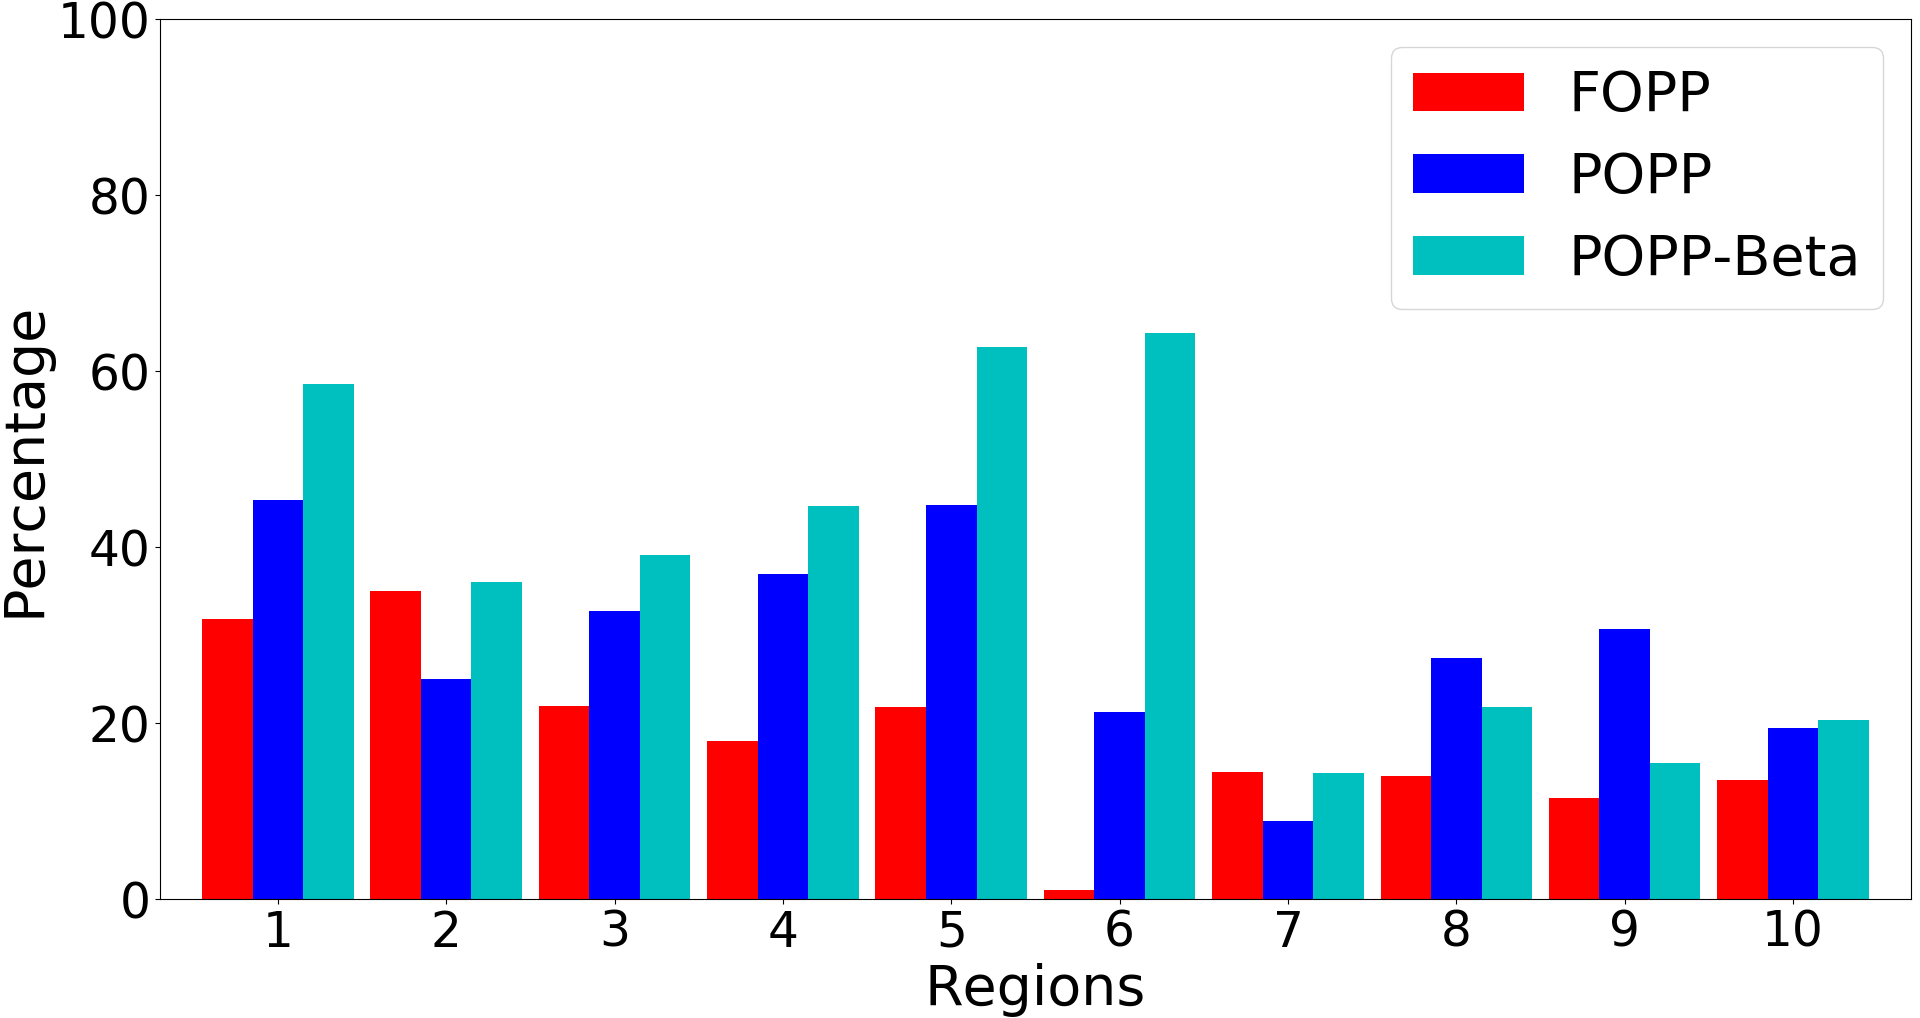
\includegraphics[width=0.5\textwidth]{./figures/exploration_percentage_region.png}
	\caption{This graph shows the percentage of time that the robot observed activities when it was present in a region. It is a measure of how successful the robot's visit policy (choice of visit time and visit location) was in finding people. It presents results for for the FOPP, POPP and POPP-algorithms. %The activity exploration percentage across areas of the environment using three different exploration models (FOPP, POPP, POPP-Beta). The percentage shows the portion of time that the robot was observing activities.
	}
	\label{fig:exploration_percentage_region}
\end{figure}

%\begin{figure}[t!]
%	\centering
%	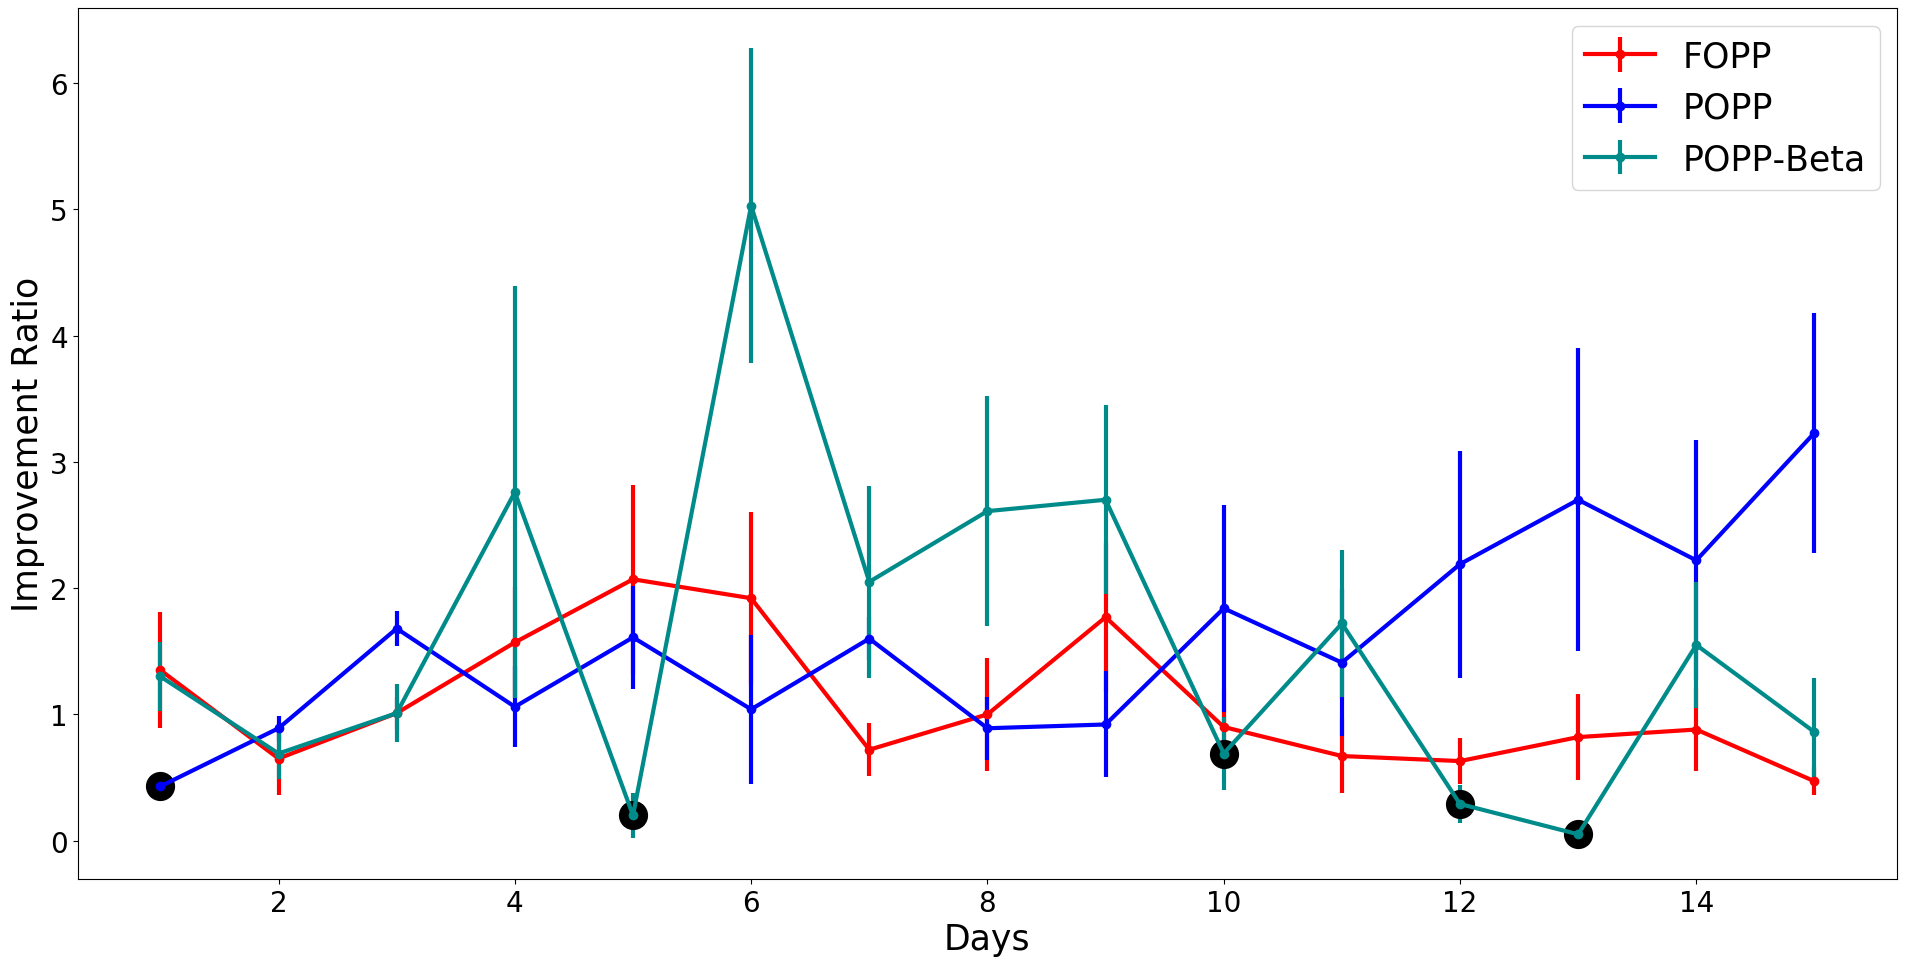
\includegraphics[width=0.5\textwidth]{./figures/exploration_improvement_ratio.png}
%	\caption{The improvement evolution of activity observation (in ratio) using three different exploration models. The average of the first three days of the number of observations on each exploration is used as the base (ratio 1.0). Black dots represent weekends the explorations were passing through.}
%	\label{fig:exploration_improvement_ratio}
%\end{figure}

%\begin{figure}[t!]
%	\centering
%	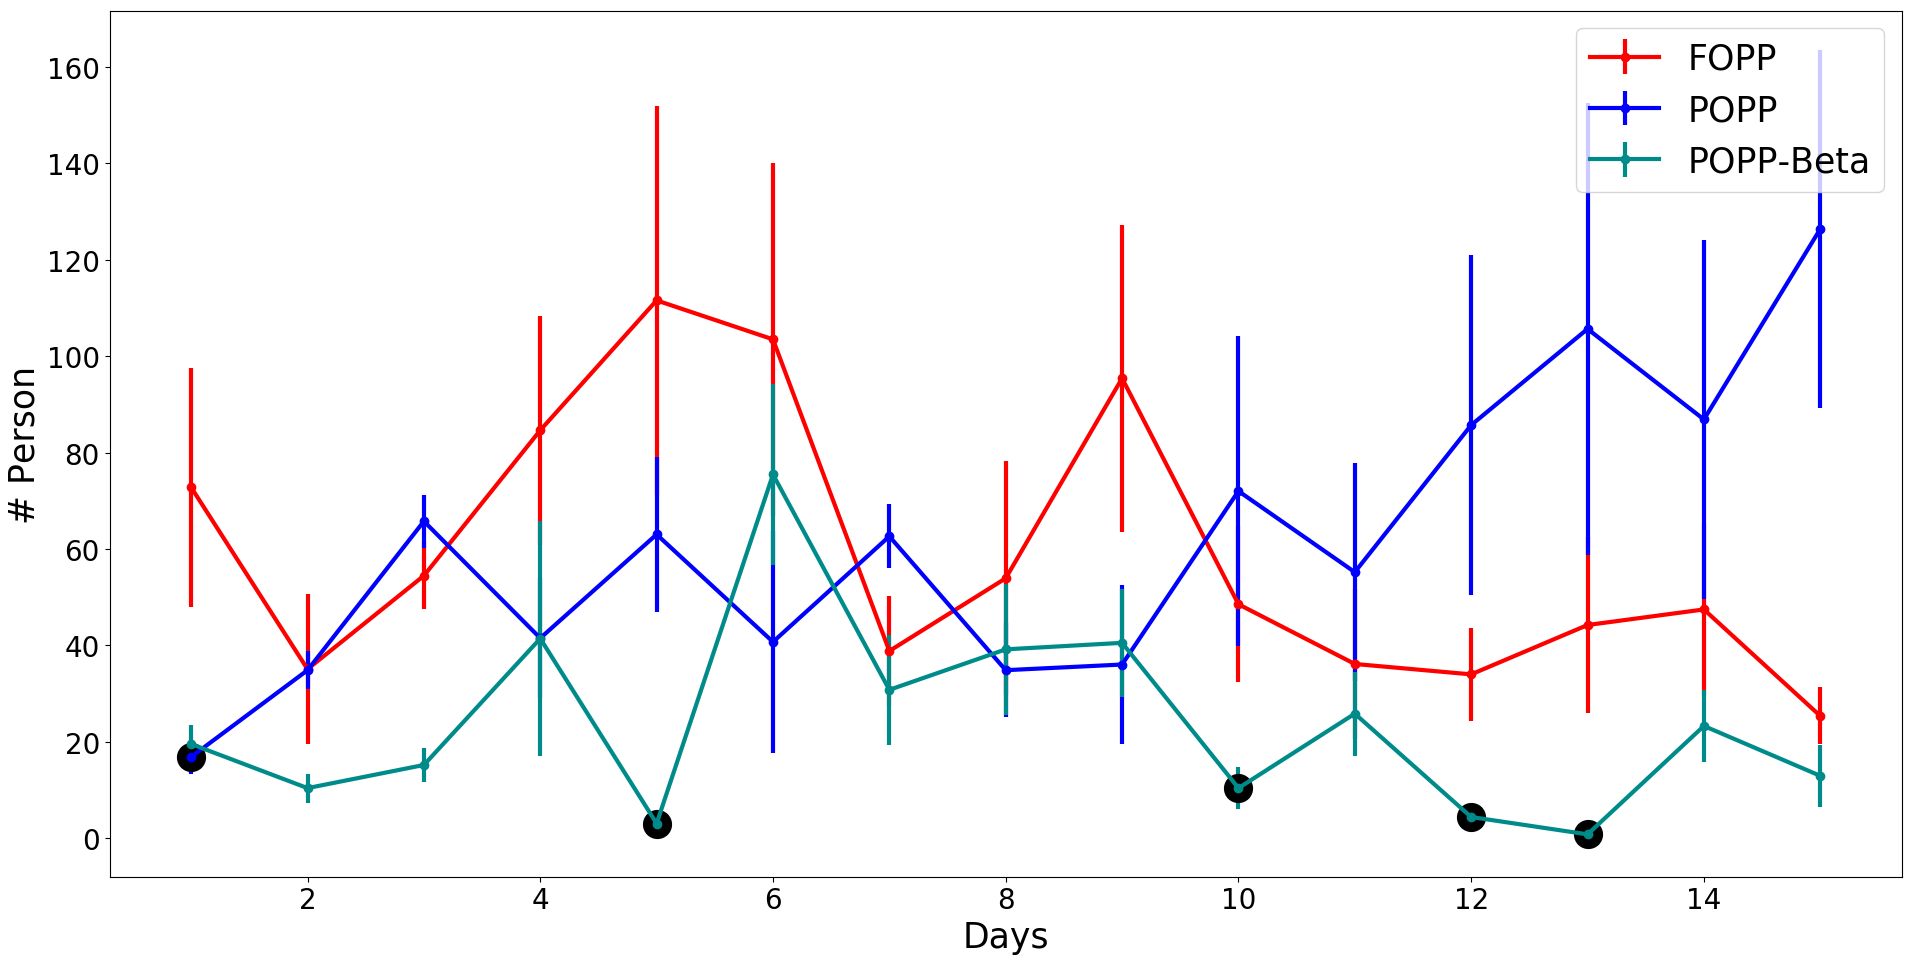
\includegraphics[width=0.5\textwidth]{./figures/exploration_number_people_across_days.png}
%	\caption{Average number of activities observed over days across regions. Black dots represent weekends the explorations were passing through.}
%	\label{fig:exploration_number_people_across_days}
%\end{figure}

\begin{figure}[t!]
	\centering
	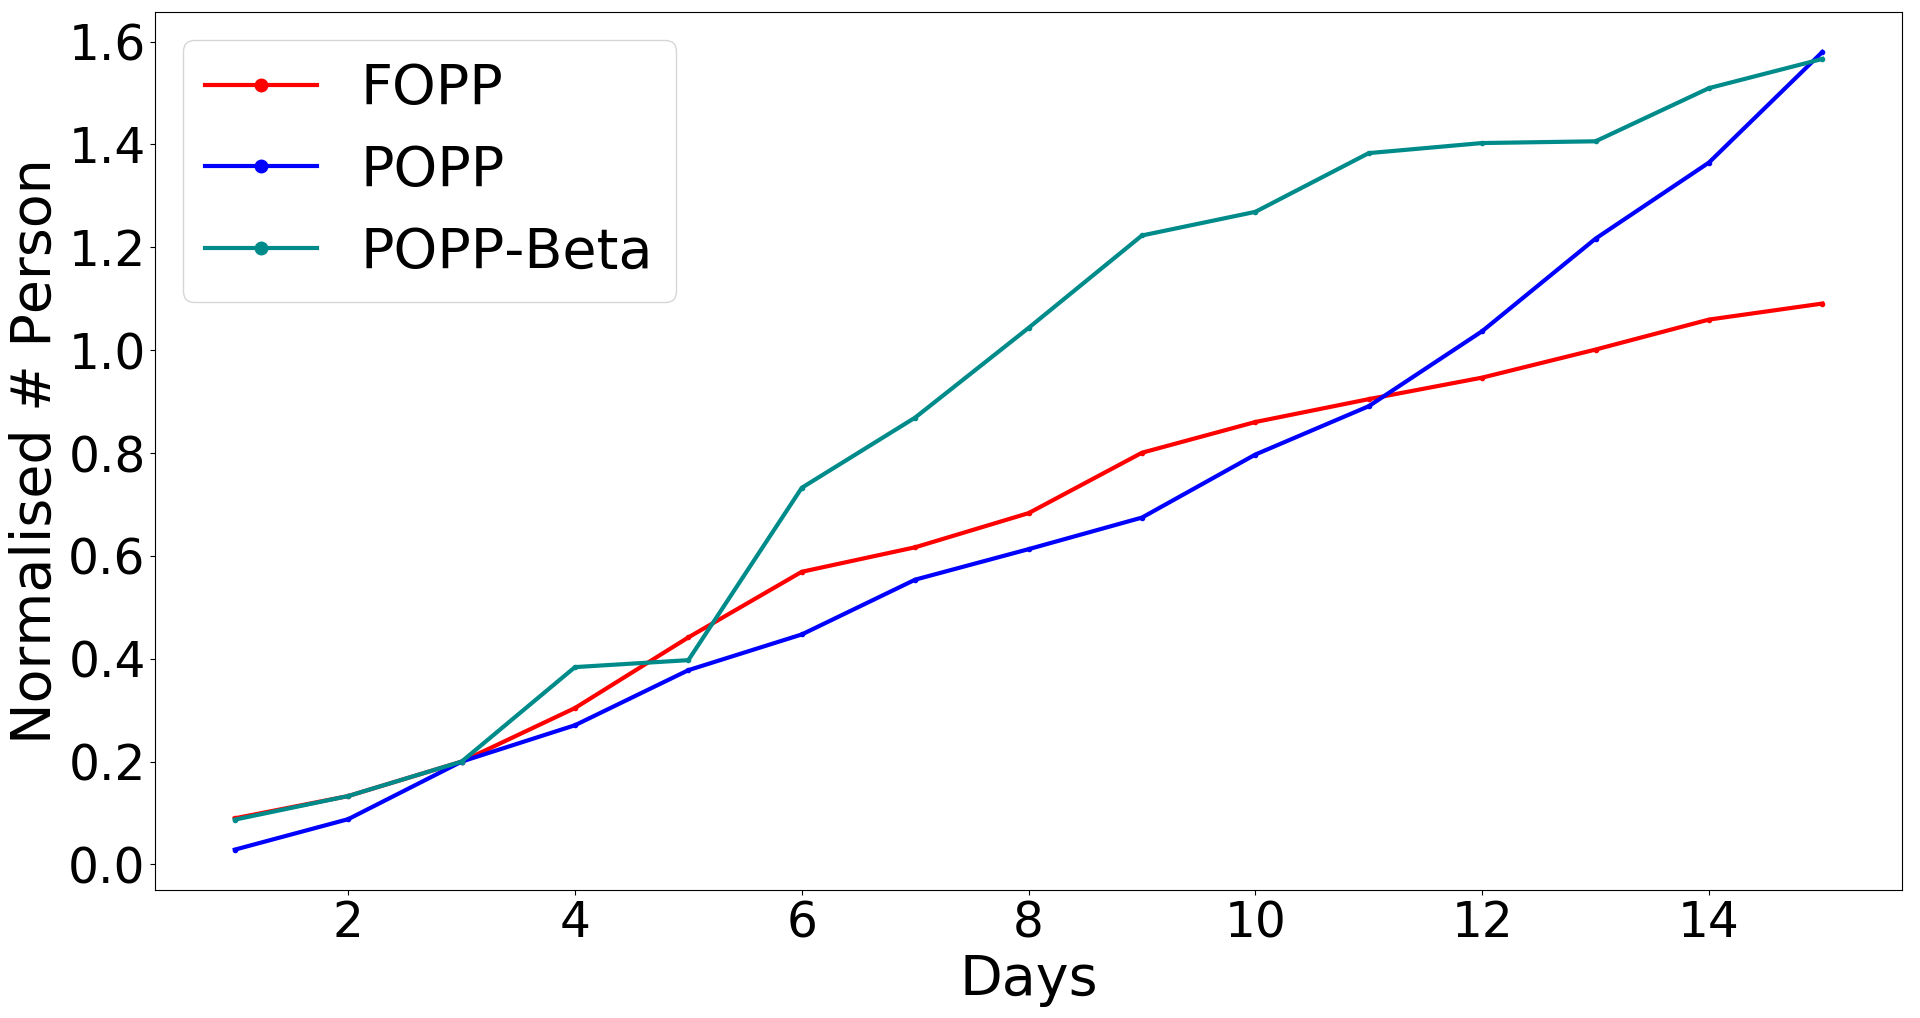
\includegraphics[width=0.5\textwidth]{./figures/exploration_number_people_across_days_normalised.png}
	\caption{The improvement ratio of activity observations during each phase of the trial. The dash line indicates a baseline performance, i.e., no improvement in exploration over time.}
	\label{fig:exploration_improvement_ratio}
\end{figure}

Figure \ref{fig:exploration_percentage_region} shows the percentage of visits to each region which yielded a non-zero true count. As can be seen, the exploration policy produced by POPP-Beta has the highest proportion of such visits in many of the regions, followed by the exploration policy according to the POPP model. Recall that some regions, such as 4, 5, 6, and 7, are not densely populated with humans across time compared to other regions (such as 1, 2, 3, and 10). The POPP and POPP-Beta models, however, still managed to improve the percentage of positive observations. This shows that the models correctly predicted that people would be present in particular locations at particular times. One should note that region 6 contains vending machines which are often detected as a person by the upper body detector. This leads to the FOPP model planning to visit this particular location when no activity is taking place. The POPP and the POPP-Beta models were able to correct the miscounts occurring in region 6, providing a better estimate of the posterior over the arrival rate $\lambda$. This leads to models that better capture the true underlying process and thus support more accurate exploration-exploitation trade-offs.

% Figure \ref{fig:exploration_number_people_across_days} shows the average number of activities observed across regions on each day. 

During the first few days of each 15 day phase the robot primarily explores since each model initially has a highly uncertain estimate of $\lambda$. As more days of data are experienced the estimates increase in confidence and the robot starts to exploit this increased confidence by visiting locations which are likely to provide higher counts\footnote{Note that this change from exploration to exploitation occurs naturally and gradually in an upper bound-based model, and therefore the characterisation of the behaviour as exploring or exploiting is a \emph{post-hoc} justification.}.
% 
To allow us to produce a metric for a fair comparison across three models (FOPP, POPP, and POPP-Beta) deployed at different times (and thus experiencing different population dynamics), we look at the ratio between the expected observations made by a baseline policy and those made by our exploration policy in the same period. 
% 
To create the baseline total for each model we take the true counts experienced for its first three days then multiply these by five to give an expected total over 15 days (the number of days of data available to every model). This is the denominator in Eqn.~\ref{eq:metric}, where $s(n)$ is the (true) number of people observed on day $n$. This is used to divide the cumulative number of observations up to the current day:

\begin{equation}
	\label{eq:metric}
\hat{s}(n) = \frac{\displaystyle\sum_{i=1}^{n} s(i)}{\displaystyle\sum_{i=1}^{3} s(i) * 5}
\end{equation}

\noindent Given this, a $\hat{s}$ score of 1.0 on day 15 shows that people have been observed people at the rate of the baseline, i.e.\ the underlying model has failed to exploit additional data correctly. A result over 1.0 shows that the model has exploited the available data to observe people at a greater rate than in the first 3 days. 
% 
Figure \ref{fig:exploration_improvement_ratio} presents the cumulative normalised true counts of people observed by the robot across the three phases. This shows that exploration driven by the POPP and the POPP-Beta models improves the number of people observed during these phases. By the end of each of these two phases, the ratio is around 1.7. On the other hand, the FOPP showed a stable ratio around the baseline (1.0 at day 15), this means that the FOPP is not be able to improve the number of people observed over time. 
% 
Also note the general trend observed earlier that the approach which represents the uncertainty in the sensor models (POPP-Beta) initially out-perform less informed approach (POPP) until the latter has observed enough of the underlying process to compensate for training inaccuracies. 

%Unfortunately for the POPP-Beta, by looking at figure \ref{fig:exploration_improvement_ratio}, we can not conclude whether the POPP-Beta can improve the number of activities observed over time.
%We argue that this is because the exploration policy produced by the Specctral-POPP-Beta was running through several weekends. We assumed of daily periodicities for the non-homogeneous Poisson processes across regions, and the assumption was broken by running the exploration throughout weekends. This is because weekdays and weekend have different arrival rate $\lambda$. Figure \ref{fig:exploration_number_people_across_days} clearly shows how small the total activities observed during weekend compared to weekdays.
\section{Conclusion}
\label{sec:conclusion}

This work has been concerned with developing practical estimators for count data collected by an autonomous mobile robot, with unreliable perception algorithms. These count data represent the level of human activity in particular locations. This work extends the work in \cite{jovan18a} with several contributions:

\begin{itemize} 
    % \item A set of inference methods for the partially observable Poisson process (POPP) has been formulated. The POPP is a Poisson process which takes into account the unreliability of the sensors that count events. Unlike Bayesian estimation for a fully observable Poisson process (FOPP), obtaining the posterior is non-trivial, since there is no conjugate density for a POPP and the posterior has a number of elements that grow exponentially in the number of observed intervals. Two simple, tractable, approximations have been presented. These two approximations are combined in a switching filter, which enables efficient and accurate estimation of the posterior. A simulation study shows that these POPP filters correct the over- and under-counts produced by sensors.  
    \item Variations of the POPP filter are presented. The POPP-Beta filter extends the POPP filter in which the unreliability of the observation model is accounted for when estimations are built. The N-POPP filter extends the POPP filter by modelling the case when sensors are uncorrelated. The POPP-Dirichlet combines the POPP-Beta filter and the N-POPP filter to have the benefits of each correction. A simulation and observations taken by a robot, on a series of long deployments, show that each extension provides progressively more accurate estimates than the POPP filter.  
    \item Both posteriors from the Spectral-FOPP and two Spectral-POPP processes are used to drive exploration by a mobile robot for a series of two week deployments. An upper bound interval exploration method was used to solve the exploration-exploitation problem. After labelling by humans, this resulted in a labelled data set of six weeks of human activity levels. A simulated study has shown that the Spectral-FOPP and the Spectral-POPP filter improve on-point observation time significantly if strong periodic patterns underlying the human activities are present. 
\end{itemize}
        
        % Finally, the various POPP filters are compared to one another and to a FOPP estimator on this data set.

% which capture the regular structures of dynamic behaviours, especially humans,    
% 
% 
% Hence, any learning algorithm requires practical estimation which capture temporal structures of human activities.   
% 
% The adaptation requires practical estimation which capture the structure 
% 
% The robot will be able to demonstrate that it can recognise activities at various
% temporal scales, and infer or predict future activities based on its temporal model (e.g. it
% might go to the lounge because it has just seen the residents finishing their lunch). It
% will also be able to detect anomalies as sequences of very low likelihood data.
% 
% The robot only observes a limited portion of the space at any time, and so must actively plan to go to places to observe events.
% 
% learns dynamic behaviours of its surrounding while patroling around perimeters of a large area. 
% 
% Human activities follow predictable, repeating patterns that generate corresponding
% changes in space.
% 
% Our
% work will allow a robot to create a map of a building and its contents: not just walls but people,
% furniture and objects, all in a unified spatial-temporal representation that will allow a robot to
% respond robustly to the dynamics of its environment. In order to reason about the structure
% and purpose of these dynamics we will employ the spatial-temporal representations in support of
% activity recognition. This will allow the robot to detect, and exploit, patterns of human behaviour.
% 
% In our care scenario we will explore how a robot can support staff working with a small group of
% elderly patients in a nursing facility. The robot will learn about the patients’ regular activities. It
% will use this knowledge to perform support tasks for the care staff and serve as an early warning
% system when patients vary from regular behaviour (e.g. wandering the corridors at night, falling
% over). In our security scenario we will explore how a robot can act as a security guard, performing
% patrols to learn the typical spatial-temporal structures in a building and notifying a human guard
% of suspicious variations from these.

% \section{Limitations and Further Work}
% 
% Two basic statistical models: Spectral-FOPP and POPP  have been proposed and evaluated. The combination of these two is able to extract temporal dynamics in the aggregate level of human activities from unreliable sensors, along with the ability to exploit this understanding for better exploration by an autonomous mobile robot. However, the spectral-POPP model could still be improved in the following two ways:
% \begin{enumerate}
%     \item In Chapter \ref{chap:popp_independent}, The Gamma filter approximates a sum of Gamma distributions with a single Gamma distribution assuming that the sensor performs rather reliable. Instead of using a single Gamma distribution to approximate a sum of $m$ Gamma distributions, $n$ gamma distributions, where $n$ is much smaller than $m$, could be used to improve the accuracy of the approximation to the posterior. This would promise to be more accurate than a single gamma, but more efficient than a histogram filter. Thus, it might be faster than the switching filter.
% 
%     \item The spectral-Poisson model (Spectral-FOPP) in Chapter \ref{chap:spectral_poisson} is a statistical model which is able, and only able, to capture the periodic structure of count data. It indirectly assumes that there is an underlying pattern governing the evolution of the parameter $\lambda$ of a Poisson process. The spectral-Poisson might not be able to capture other non-periodic structures governing the parameter $\lambda$, such as trends. 
% 
%         A Gaussian process modulated Poisson process might provide a better model for different structures which govern $\lambda$ overtime. Work from \cite{lloyd2015variational} presents a fully variational Bayesian inference scheme for continuous Gaussian-process modulated Poisson process. It provides a good estimators and is fast in estimating $\lambda$ of a Poisson process. An extension to this statistical model which embeds both trends and periodicity in the model might provide a solution to the limitations of Spectral-Poisson while being fully Bayesian. 
% \end{enumerate}

% Listing all limitations which have been mentioned in previous sections.
% Listing all further work which can extend this thesis.

\ifCLASSOPTIONcompsoc
  \section*{Acknowledgments}

\else
  \section*{Acknowledgment}
\fi

The research leading to these results has received funding from the European Union Seventh Framework Programme (FP7/2007-2013) under grant agreement No 600623, STRANDS.

%!TEX root = ../bare_jrnl.tex

\appendices
\label{sec:supplementary}
\section{Sensor Model}

Here we provide detailed sensor models for each region. The sensor model was built from the first 15 days of data to give a general idea how each sensor performs across days. For the experiment in Section \ref{sec:evareal}, we used 48 days of data, and as we performed four fold cross validation, we only used 12 days of data to build the sensor model. During the exploration setting, only the first 3 days from 15 days of exploration for each exploration model were used to build the sensor model.

\begin{table}[h]
	\centering
	\caption{Averaged sensor model for each region trained from 15 days of data.}
	\label{table:full_region_sensor_model}
	\begin{tabular}{llccc}
		\noalign{\hrule height 1.1pt}\noalign{\smallskip}
		Region & Sensor & True Negative & True Positive \\
		\noalign{\smallskip}\hline\noalign{\smallskip}
		1   & Leg               & 0.820 & 0.102 \\
		& Upper body        & 0.749 & 0.244 \\
		& Scenery change    & 0.760 & 0.612 \\ 
		2   & Leg               & 0.991 & 0.655 \\
		& Upper body        & 0.862 & 0.691 \\
		& Scenery change    & 0.826 & 0.778 \\
		3   & Leg               & 0.854 & 0.116 \\
		& Upper body        & 0.833 & 0.130 \\
		& Scenery change    & 0.780 & 0.687 \\
		4   & Leg               & 0.896 & 0.180 \\
		& Upper body        & 0.967 & 0.227 \\
		& Scenery change    & 0.897 & 0.592 \\
		5   & Leg               & 0.918 & 0.086 \\
		& Upper body        & 0.881 & 0.200 \\
		& Scenery change    & 0.877 & 0.957 \\
		6   & Leg               & 0.964 & 0.351 \\
		& Upper body        & 0.929 & 0.143 \\
		& Scenery change    & 0.803 & 0.541 \\
		7   & Leg               & 0.949 & 0.264 \\
		& Upper body        & 0.829 & 0.071 \\
		& Scenery change    & 0.939 & 0.090 \\
		8   & Leg               & 0.889 & 0.473 \\
		& Upper body        & 0.791 & 0.360 \\
		& Scenery change    & 0.900 & 0.591 \\
		9   & Leg               & 0.702 & 0.383 \\
		& Upper body        & 0.711 & 0.172 \\
		& Scenery change    & 0.591 & 0.673 \\
		10  & Leg               & 0.956 & 0.537 \\
		& Upper body        & 0.973 & 0.423 \\
		& Scenery change    & 0.823 & 0.584 \\
		%\multirow{2}{*}{Method} & \multicolumn{3}{c}{Average updating time (std. deviation)} \\
		%& 100 & 1000  & 10000 \\
		\noalign{\hrule height 1.1pt}\noalign{\smallskip}
	\end{tabular}
\end{table}

\section{Discrete Probability Distribution}

%\begin{definition2}
%	A random variable $X$ is a Bernoulli random variable with parameter $p$, i.e. $X \sim Ber(x ; p)$, if its probability mass function is given by
%	\[
%	Ber(x ; p) = \left\{ \begin{matrix}
%	p & \textrm{if } x = 1 \\
%	1-p & \textrm{if } x = 0 % \\
%	% 0 & \textrm{otherwise}
%	\end{matrix} \right.
%	\]
%	\noindent where $0 \leq p \leq 1$ and $x \in \{0, 1\}$.
%\end{definition2}
%
%\begin{definition2}
%	A random variable $X$ is a binomial random variable with parameter $n$ and $p$, i.e. $X \sim B(x ; n, p)$, if its probability mass function is given by
%	\[
%	B(x ; n, p) = \begin{pmatrix} n \\ x \end{pmatrix} p^x (1-p)^{n-x}
%	\]
%	\noindent where $0 \leq p \leq 1$ and $x \in \{0, \ldots, n\}$.
%\end{definition2}

\begin{definition2}
	A random variable $X$ is a negative binomial random variable with parameter $n$ and $p$, i.e. $X \sim NB(x ; n, p)$, if its probability mass function is given by
	\[
	NB(x ; n, p) = \begin{pmatrix} x - 1 \\ n - 1 \end{pmatrix} p^n (1 - p)^{x-n}
	\]
	\noindent where $0 \leq p \leq 1$ and $x \geq n$.
\end{definition2}

\begin{definition2}
	A random variable $X$ is a beta-binomial random variable with parameter $n, \zeta, \eta$, i.e. $X \sim BB(x ; n, \zeta, \eta)$ where the $p$ parameter in the binomial distribution $B(x ; n, p)$ is randomly drawn from a beta distribution $Be(p ; \zeta, \eta)$ 
	\begin{equation*}
	\begin{tabular}{r@{ = }l}
	$P(x ; n, \zeta, \eta)$ & $\displaystyle\int_{p=0}^{1} P(x ; n, p) ~ P(p ; \zeta, \eta) ~dp$ \\ [2ex]
	& $\displaystyle\int_{p=0}^{1} B(x ; n, p) ~ Be(p ; \zeta, \eta) ~dp$ \\ [2ex]
	& $\displaystyle\int_{p=0}^{1} \binom{n}{x} p^x (1-p)^{(n-x)} ~ \displaystyle\frac{p^{(\zeta - 1)} (1-p)^{(\eta-1)}}{\pi(\zeta, \eta)}$ \\ [2ex]
	& $\displaystyle\binom nx \displaystyle\frac{1}{\pi(\zeta, \eta)} ~ \displaystyle\int_{p=0}^{1} p^{(x+\zeta-1)} (1-p)^{(n-x+\eta-1)} ~dp$ \\ [2ex]
	& $\displaystyle\binom nx \displaystyle\frac{\pi(x+\zeta, n-x+\eta)}{\pi(\zeta, \eta)}$ \\ [2ex]
	& $BB(x ; n, \zeta, \eta)$
	\end{tabular}
	\end{equation*}
\end{definition2}

\begin{definition2}
	Let $\mathbf{x}$ be a vector of $x_1, \ldots, x_m$, and $\mathbf p$ be a vector of $p_1, \ldots, p_m$. A random variable $X$ is a categorical random variable with parameter $\mathbf p$, i.e. $X \sim Cat(\mathbf x ; \mathbf p)$, if its probability mass function is given by
	\[
	Cat(\mathbf x ; \mathbf p) = \begin{matrix}
	p_i & \textrm{if } x_i = 1 \\
	\end{matrix}.
	\]
	\noindent where $x_i = \{0, 1\}$ and $\displaystyle\sum_{i=1}^{m} p_i = 1$.
\end{definition2}

\begin{definition2}
	Let $\mathbf{x}$ be a vector of $x_1, \ldots, x_m$, and $\mathbf p$ be a vector of $p_1, \ldots, p_m$. A random variable $X$ is a multinomial random variable with parameter $n$ and $\mathbf p$, i.e. $X \sim Multi(\mathbf x ; n, \mathbf p)$, if its probability mass function is given by
	\[
	Multi(\mathbf x ; n, \mathbf p) = \begin{array}{lll}
	\displaystyle \frac{n!}{x_1!, \ldots, x_m!} p^{x_1}_1 \times \ldots \times p^{x_m}_m, \\ 
	\end{array}
	\]
	\noindent where $x_i = 0, 1, \ldots$, $\displaystyle\sum_{i=1}^{m} x_i = n$, $0 \leq p_i \leq 1$, $i = 1, \ldots, m$ and $\displaystyle\sum_{i=1}^{m} p_i = 1$.
\end{definition2}

% An example of a double column floating figure using two subfigures.
% (The subfig.sty package must be loaded for this to work.)
% The subfigure \label commands are set within each subfloat command,
% and the \label for the overall figure must come after \caption.
% \hfil is used as a separator to get equal spacing.
% Watch out that the combined width of all the subfigures on a 
% line do not exceed the text width or a line break will occur.
%
%\begin{figure*}[!t]
%\centering
%\subfloat[Case I]{\includegraphics[width=2.5in]{box}%
%\label{fig_first_case}}
%\hfil
%\subfloat[Case II]{\includegraphics[width=2.5in]{box}%
%\label{fig_second_case}}
%\caption{Simulation results for the network.}
%\label{fig_sim}
%\end{figure*}
%
% Note that often IEEE papers with subfigures do not employ subfigure
% captions (using the optional argument to \subfloat[]), but instead will
% reference/describe all of them (a), (b), etc., within the main caption.
% Be aware that for subfig.sty to generate the (a), (b), etc., subfigure
% labels, the optional argument to \subfloat must be present. If a
% subcaption is not desired, just leave its contents blank,
% e.g., \subfloat[].


% An example of a floating table. Note that, for IEEE style tables, the
% \caption command should come BEFORE the table and, given that table
% captions serve much like titles, are usually capitalized except for words
% such as a, an, and, as, at, but, by, for, in, nor, of, on, or, the, to
% and up, which are usually not capitalized unless they are the first or
% last word of the caption. Table text will default to \footnotesize as
% the IEEE normally uses this smaller font for tables.
% The \label must come after \caption as always.
%
%\begin{table}[!t]
%% increase table row spacing, adjust to taste
%\renewcommand{\arraystretch}{1.3}
% if using array.sty, it might be a good idea to tweak the value of
% \extrarowheight as needed to properly center the text within the cells
%\caption{An Example of a Table}
%\label{table_example}
%\centering
%% Some packages, such as MDW tools, offer better commands for making tables
%% than the plain LaTeX2e tabular which is used here.
%\begin{tabular}{|c||c|}
%\hline
%One & Two\\
%\hline
%Three & Four\\
%\hline
%\end{tabular}
%\end{table}

\ifCLASSOPTIONcaptionsoff
  \newpage
\fi

% trigger a \newpage just before the given reference
% number - used to balance the columns on the last page
% adjust value as needed - may need to be readjusted if
% the document is modified later
%\IEEEtriggeratref{8}
% The "triggered" command can be changed if desired:
%\IEEEtriggercmd{\enlargethispage{-5in}}

% REFERENCES
\bibliographystyle{IEEEtran}
\bibliography{biblio}

% biography section with photo
%\begin{IEEEbiography}[{\includegraphics[width=1in,height=1.25in,clip,keepaspectratio]{mshell}}]{Michael Shell}
% \begin{IEEEbiography}{Ferdian Jovan}
% Biography text here.
% \end{IEEEbiography}

% biography section without photo
\begin{IEEEbiographynophoto}{Ferdian Jovan}
Biography text here.
\end{IEEEbiographynophoto}

\begin{IEEEbiographynophoto}{Jeremy Wyatt}
Biography text here.
\end{IEEEbiographynophoto}

\begin{IEEEbiographynophoto}{Nick Hawes}
Biography text here.
\end{IEEEbiographynophoto}

% % insert where needed to balance the two columns on the last page with
% % biographies
% %\newpage
% 
% \begin{IEEEbiographynophoto}{Jane Doe}
% Biography text here.
% \end{IEEEbiographynophoto}

% You can push biographies down or up by placing
% a \vfill before or after them. The appropriate
% use of \vfill depends on what kind of text is
% on the last page and whether or not the columns
% are being equalized.

%\vfill

% Can be used to pull up biographies so that the bottom of the last one
% is flush with the other column.
%\enlargethispage{-5in}

\end{document}
